% !TeX program = lualatex
% UTF-8 source. Compile twice with LuaLaTeX.
% Keep the figures/ directory alongside this .tex when copying the report.
% All tables use booktabs: top rule, header mid rule, bottom rule only.
% Benchmark records below belong to their stated historical snapshots.
% This .tex is the authoritative editable report; do not regenerate from older builders.
\documentclass[UTF8,a4paper,10pt,twocolumn,fontset=fandol]{ctexart}
\usepackage[margin=1.65cm,top=1.75cm,bottom=1.75cm]{geometry}
\usepackage{booktabs,tabularx,array,longtable}
\usepackage{amsmath,graphicx}
\usepackage{xcolor}
\usepackage{caption}
\usepackage{fancyhdr,lastpage}
\usepackage{seqsplit}
\usepackage[unicode,hidelinks]{hyperref}
\hypersetup{pdftitle={LevelDB TTL 与统计元数据实验报告},pdfauthor={周光轩；唐一嘉}}
\definecolor{diagramblue}{HTML}{365C75}
\setlength{\columnsep}{0.8cm}
\setlength{\parindent}{2em}
\setlength{\parskip}{0.25em}
\setlength{\emergencystretch}{2em}
\linespread{1.20}
\raggedbottom
\setlength{\textfloatsep}{10pt plus 2pt minus 2pt}
\setlength{\intextsep}{8pt plus 2pt minus 2pt}
\setlength{\floatsep}{8pt plus 2pt minus 2pt}
\ctexset{
 section={format=\heiti\large,beforeskip=1.1em,afterskip=0.55em},
 subsection={format=\heiti\normalsize,beforeskip=0.8em,afterskip=0.4em}
}
\captionsetup{font=small,labelfont=normalfont,labelsep=quad,skip=5pt}
\pagestyle{fancy}
\fancyhf{}
\fancyhead[L]{\footnotesize 数据库系统课程实验 · Project 1}
\fancyhead[R]{\footnotesize LevelDB TTL 与统计元数据}
\fancyfoot[C]{\footnotesize\thepage\ / \pageref{LastPage}}
\setlength{\headheight}{14pt}
\renewcommand{\headrulewidth}{0.4pt}
\renewcommand{\footrulewidth}{0pt}
\newcolumntype{Y}{>{\raggedright\arraybackslash}X}
\setcounter{topnumber}{3}
\renewcommand{\topfraction}{0.9}
\renewcommand{\textfraction}{0.05}
\renewcommand{\floatpagefraction}{0.8}
\renewcommand{\dbltopfraction}{0.9}
\begin{document}
\twocolumn[{
\begin{center}
{\heiti\LARGE LevelDB TTL 与统计元数据}\par\smallskip
{\heiti\large 实验设计 实现与验证报告}\par\medskip
{\small\url{https://github.com/Daydream709/LevelDB_Project1}}\par\medskip
周光轩\qquad 唐一嘉\par\smallskip
{\small 2026 年 11 月 5 日}
\end{center}
\begin{minipage}{\textwidth}
\linespread{1.30}\small
\noindent\textbf{摘要}\quad 本实验在 LevelDB 中实现记录有效期（TTL）和当前内部记录统计，并处理两项功能在写入、读取、回收与恢复过程中的一致性。TTL 将绝对截止时间随记录持久化，以固定的序列号和时间确定读取视图，并通过合并安全回收过期记录。统计以当前主数据为依据，增量维护记录总数、去重键数和序列号；局部计数索引辅助判断回收后的键数变化，统计与文件变更在相应提交边界发布。课程公开测试及性能对照共完成 372 次场景运行，当前实现的固定版本原生回归三轮均通过。10 万键场景下，当前实现的单线程写入和八线程并发写入吞吐分别为 482,424 和 163,066 次/s。实验也观察到部分小规模配置的吞吐下降；畸形日志恢复和自动回收估计仍有待完善。


\end{minipage}\vspace{1.3em}
}]

\section*{1 项目目标与需求分析}
LevelDB 使用日志、内存表和有序字符串表（SST）保存数据，并通过合并回收不再需要的记录。本实验在同一引擎中增加 TTL 和统计接口，重点解决读取可见性、物理记录数量与持久化状态之间的一致性问题。

\subsection*{1.1 实验任务}
我们在同一份 LevelDB 源码中完成 TTL 和统计元数据功能。TTL 解决记录何时失效、何时可以回收的问题；统计接口描述数据库当前保存的内部记录规模。两者共用写入、版本管理与合并流程，因此需要统一设计提交边界，而不能只分别实现两个接口。

普通 Put 保持永久有效；带 TTL 的 Put 接收秒数并保存绝对截止时间。到期后 Get 返回 NotFound，迭代器跳过记录。快照还需固定读取时间，避免同一快照随时间推移改变结果。本文到期语义以配置的 Env 时间为准；系统时钟回拨时，尚未物理删除的值可能重新满足未到期条件，当前实现没有额外的单调到期保证。

\subsection*{1.2 统计口径}
GetCurrentStats 返回 total\_entries、distinct\_keys 和 seq。total\_entries 统计 MemTable、Immutable MemTable 和当前 Version 中 SST 的内部记录；同一键的多个版本及删除标记分别计数。distinct\_keys 按用户键原始字节去重，seq 表示对应状态的最新已发布序列号。

用 $R(k)$ 表示当前发布状态中原始用户键 $k$ 的内部记录数，记 $T=\texttt{total\_entries}$、$D=\texttt{distinct\_keys}$、$S=\texttt{seq}$，则 $T=\sum_k R(k)$，$D=|\{k:R(k)>0\}|$。$S$ 标识与这组统计对应的写入进度，并非当前记录数。

过期只改变读取可见性，不立即减少物理统计。只有内部记录实际回收并成功安装新 Version 后，统计值才减少。WAL 是恢复副本，不重复计入。统计查询忽略 ReadOptions::snapshot，始终返回当前状态。

这里的“物理记录”限定于当前发布状态，并非磁盘上所有尚未删除的 SST；仅被旧迭代器引用的历史 Version 文件不再重复计数。删除不存在的键也会新增删除标记，因此可使记录数与去重键数同时增加。若自定义比较器将 A 与 a 判等，两种原始字节仍分别计入 distinct\_keys；这与 Get 的比较器等价语义不同。

\subsection*{1.3 设计约束}
本实验保留 LevelDB 的 LSM 存储路径。扩展必须兼容普通写入、删除、WriteBatch、自定义比较器与恢复流程，并对零 TTL、时间溢出、快照保护以及 I/O 失败给出确定语义。


\begin{table}[!htbp]
\centering
\caption{主数据操作与统计发布的伪代码}
\label{tab:algorithm-publish}
\small\setlength{\tabcolsep}{3pt}
\renewcommand{\arraystretch}{1.12}
\begin{tabularx}{\columnwidth}{@{}rY@{}}
\toprule
行号 & 伪代码 \\
\midrule
1 & \textbf{if} 操作为用户写入 \textbf{then} \\
2 & \quad 校验批次并准备统计增量 \\
3 & \quad 追加 WAL；按需执行 Sync \\
4 & \quad 成功后插入 MemTable \\
5 & \quad 持锁发布计数与最新序列号 \\
6 & \textbf{else if} 操作为刷盘 \textbf{then} \\
7 & \quad 构建并同步 SST，安装新 Version \\
8 & \quad 保持全局记录数不变 \\
9 & \textbf{else if} 操作为合并回收 \textbf{then} \\
10 & \quad 构建输出并核对统计差分 \\
11 & \quad 安装文件变更与计数检查点 \\
12 & \quad 仅在安装成功后发布新统计 \\
\bottomrule
\end{tabularx}
\par\vspace{3pt}
\parbox{\columnwidth}{\footnotesize\raggedright\textbf{注：}按操作类型分支，刷盘与合并不必紧随每次写入。此处省略队列与锁的细节；失败操作不发布其成功统计。WAL 写入或同步失败时，重启后的实际状态仍须由恢复结果确定。}
\end{table}

逻辑上，写入先生成可恢复记录，再更新可见状态；合并先准备新文件，再切换当前版本。统计在这些成功提交的边界更新，从而与数据状态对应。表~\ref{tab:algorithm-publish} 给出按操作类型划分的伪代码，具体路径中的并发协调见第 3 节。

{\small 报告以远程仓库 \href{https://github.com/Daydream709/LevelDB_Project1}{Daydream709/LevelDB\_Project1} 的当前实现为依据，说明 TTL 回收、恢复和 SST 局部计数索引，并列出已知边界。本文先介绍 TTL 与统计的设计，再分析恢复、正确性测试和性能结果。\par}

\section*{2 TTL 功能设计与实现}
\begin{figure*}[t]
\centering
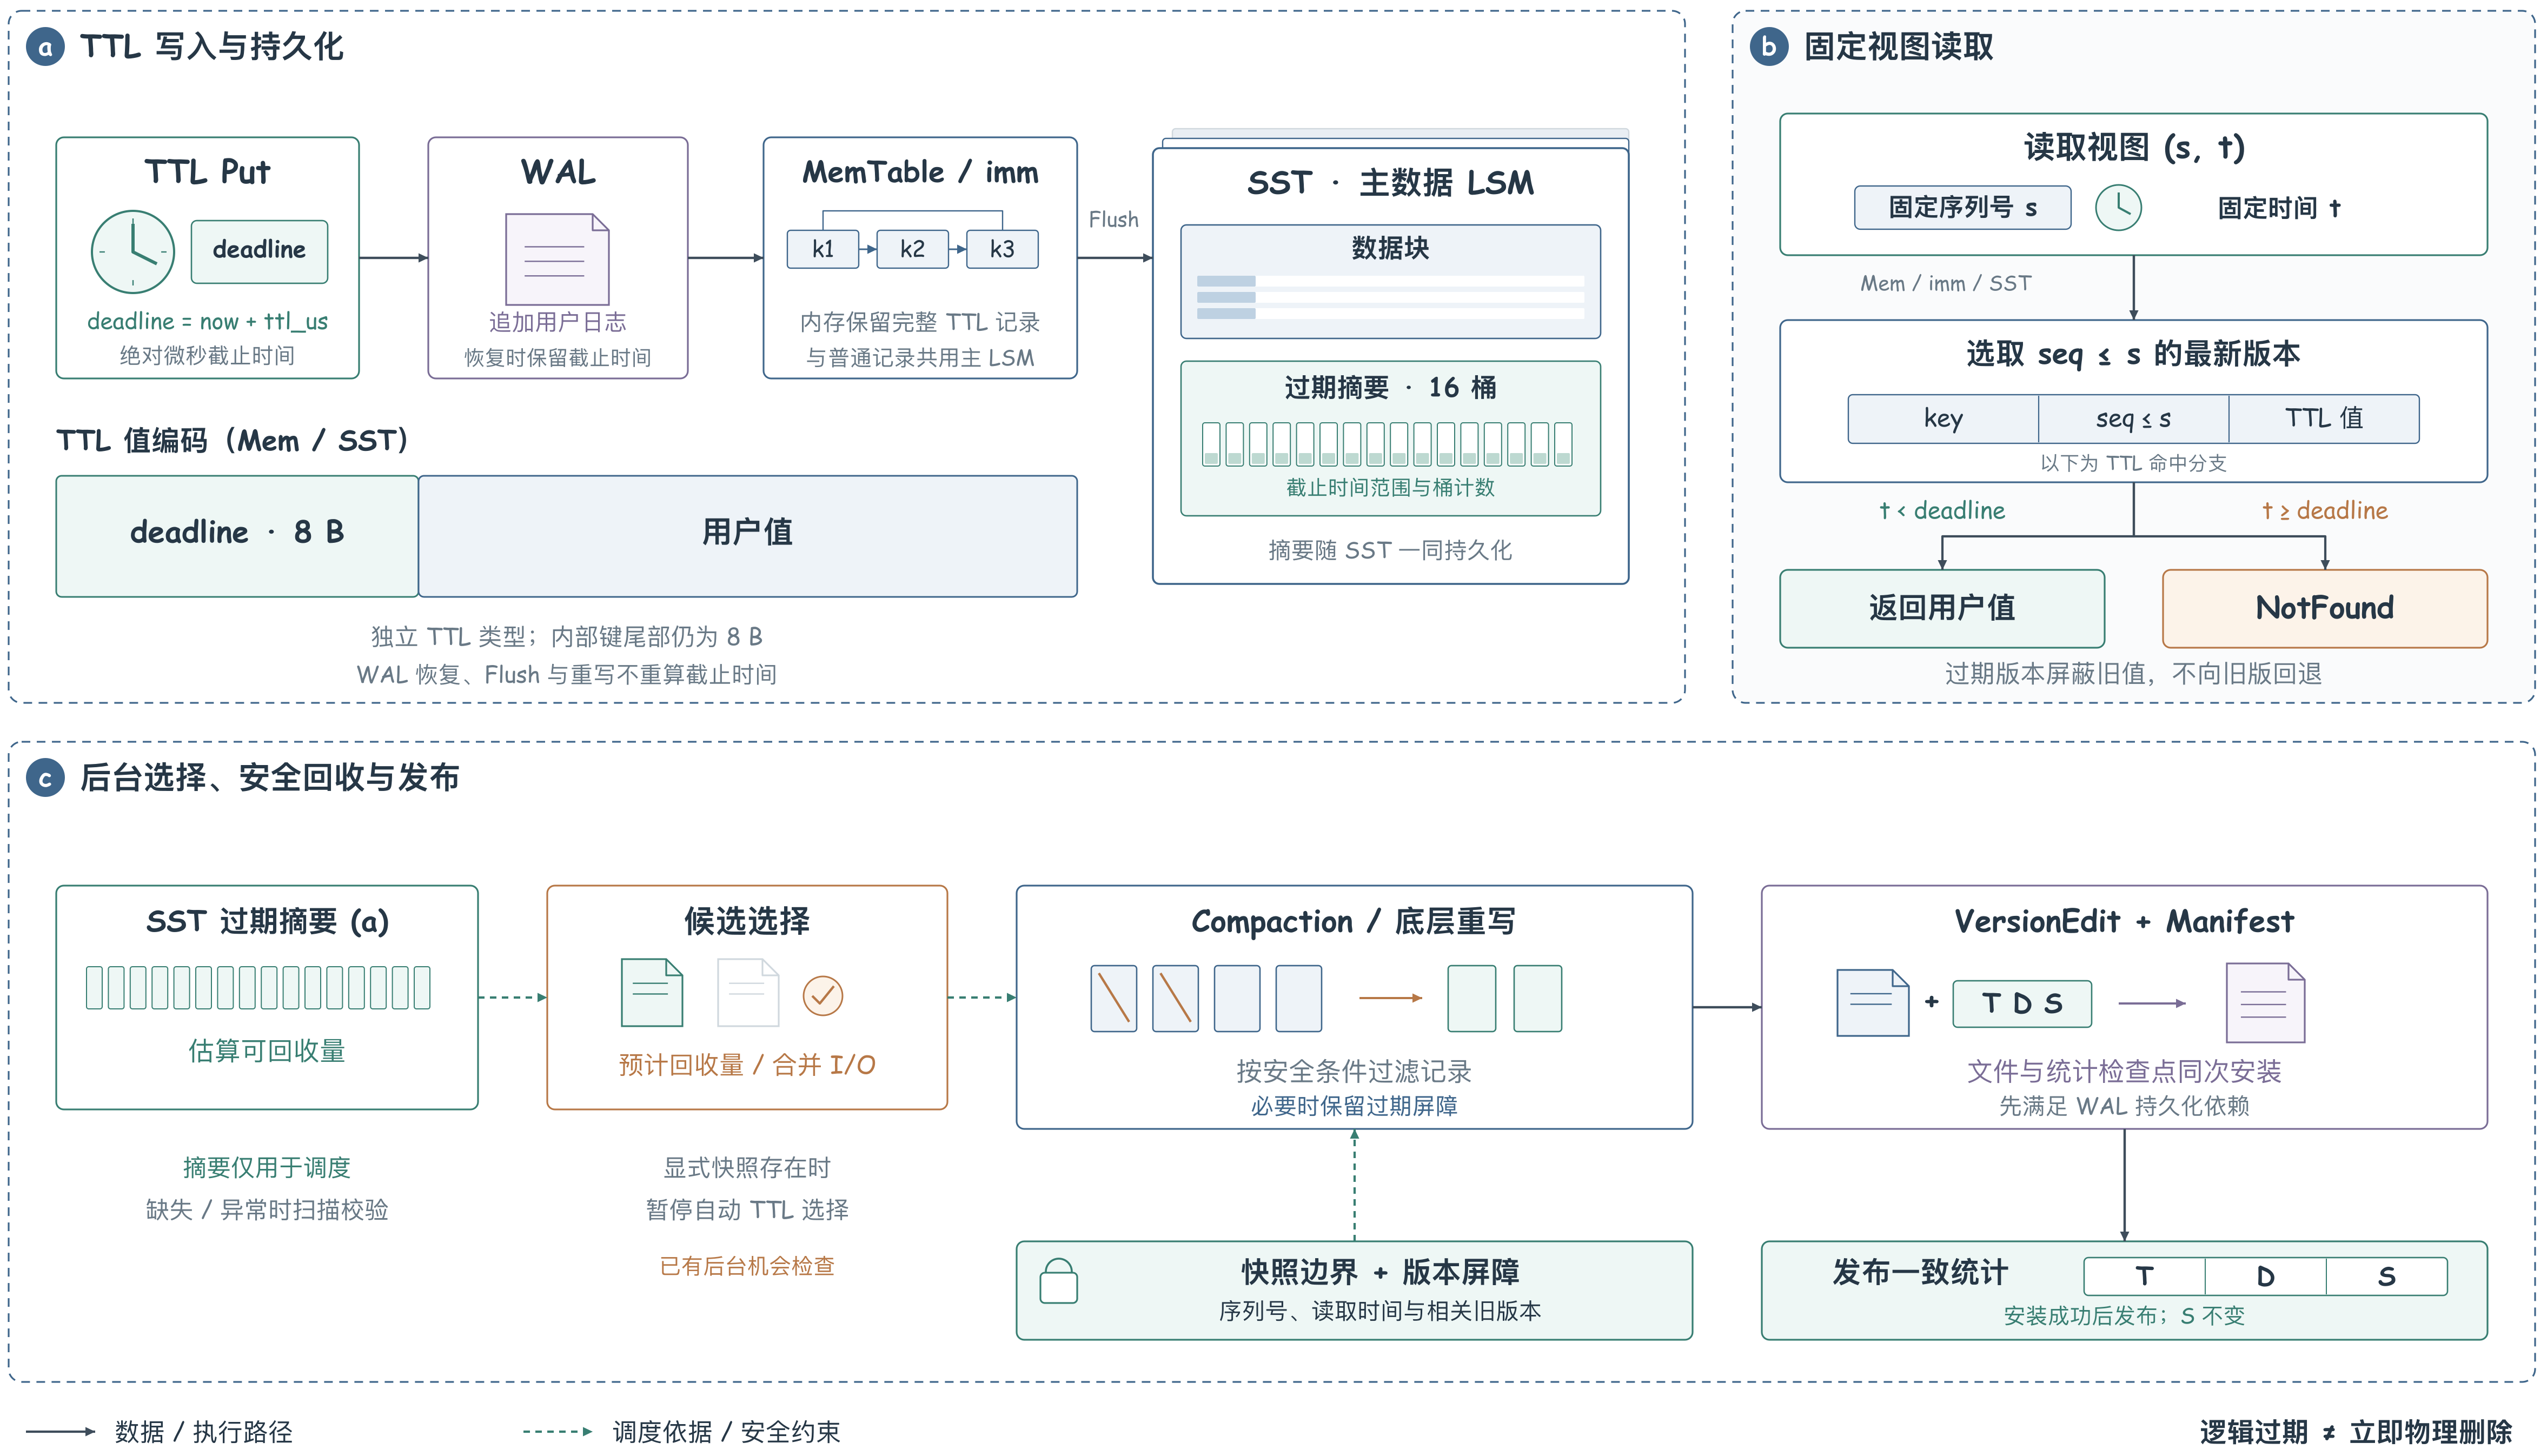
\includegraphics[width=\textwidth]{figures/ttl-overview-updated.png}
\caption{TTL 写入、固定视图读取与安全回收总览。（a）截止时间沿主数据路径持久化；（b）固定视图中的过期版本屏蔽旧值；（c）摘要用于候选调度，删除受快照和版本规则约束，文件变更与统计同次提交。读取图省略损坏载荷的错误分支；后台选择不保证按时回收。}
\label{fig:ttl-overview}
\end{figure*}
图~\ref{fig:ttl-overview} 将截止时间编码、固定读取视图和安全回收串联起来。写入与回收共用主数据路径，读可见性与物理删除分别判断。

\subsection*{2.1 编码方案与接口}
带 TTL 的 Put 通过 Options::env->NowMicros() 取得当前时间，将秒数转换为微秒，计算截止时间 $deadline=now+ttl\times 10^{6}$。实现分别检查乘法和加法溢出，错误时返回 InvalidArgument，在进入写入提交前终止，不消耗用户序列号。截止时间在进入写队列前计算，排队与 I/O 时间也计入有效期，并非写入返回成功后才开始倒计时。

ttl=0 会写入立即过期的新版本，并正常消耗序列号。它不能等同于“永久有效”，也不能直接忽略写入，否则旧值可能继续可见。永久有效的数据仍通过普通 Put 写入。


\begin{table}[htbp]
\centering
\small
\setlength{\tabcolsep}{3pt}
\renewcommand{\arraystretch}{1.25}
\caption{TTL 在不同存储层的表示}
\label{tab:report-1}
\begin{tabularx}{\columnwidth}{@{}>{\hsize=0.58000\hsize\linewidth=\hsize\raggedright\arraybackslash}X>{\hsize=1.42000\hsize\linewidth=\hsize\raggedright\arraybackslash}X@{}}
\toprule
\textbf{位置} & \textbf{编码与职责} \\
\midrule
WriteBatch / WAL & 类型标记、用户键、fixed64 截止时间、用户值 \\
InternalKey & 用户键、序列号与 kTypeValueWithTTL 类型 \\
MemTable / SST value & 8 字节绝对截止时间前缀，随后为用户值 \\
普通记录 & 保留原有 value 类型与编码 \\
\bottomrule
\end{tabularx}
\end{table}

\seqsplit{WriteBatch::PutWithExpiration} 接收绝对微秒截止时间，允许 TTL 写入与普通写入、删除放在同一原子批次。批次复制、提交和日志重放均保留原截止时间，避免恢复时重新计时。公开 Write 在入队前先校验完整批次，截断的 TTL 编码或错误操作数会返回 Corruption，不能先提交合法前缀。InternalKey 新增类型值 2，并将查找类型上界同步为该值；普通记录编码保持原样，不意味着旧版 LevelDB 能识别新增 TTL 类型。

\begin{table}[!htbp]
\centering
\caption{TTL 截止时间的溢出检查}
\label{tab:code-ttl}
\setlength{\tabcolsep}{3pt}
\renewcommand{\arraystretch}{1.05}
\begin{tabularx}{\columnwidth}{@{}r>{\ttfamily\fontsize{7.5}{9.5}\selectfont\raggedright\arraybackslash}X@{}}
\toprule
{\small 行号} & {\normalfont\small 执行语句} \\
\midrule
1 & const uint64\_t now = env\_->NowMicros(); \\
2 & const uint64\_t scale = 1000000; \\
3 & if (ttl > std::numeric\_limits<uint64\_t>::max() \\
4 & \hspace*{4.5em}/ scale) \\
5 & \hspace*{0.9em}return Status::InvalidArgument( \\
6 & \hspace*{2.7em}"TTL seconds overflow microseconds"); \\
7 & const uint64\_t ttl\_micros = ttl * scale; \\
8 & if (now > std::numeric\_limits<uint64\_t>::max() \\
9 & \hspace*{4.5em}- ttl\_micros) \\
10 & \hspace*{0.9em}return Status::InvalidArgument( \\
11 & \hspace*{2.7em}"TTL deadline overflows Env time"); \\
12 & deadline = now + ttl\_micros; \\
\bottomrule
\end{tabularx}
\par\vspace{3pt}
\parbox{\columnwidth}{\footnotesize\raggedright\textbf{注：}摘自 \texttt{db/db\_impl.cc} 的 TTL Put 路径；仅调整换行，省略外层性能计时包装。先检查秒转微秒与时间加法，失败时不进入写入提交。}
\end{table}

表~\ref{tab:code-ttl} 展示截止时间计算前的两级溢出检查。

\subsection*{2.2 读取与旧版本屏蔽}
Get 先按读取序列号定位目标键的最新可见内部版本，再判断类型和截止时间。如果该版本已过期，返回 NotFound 并结束查找，不能继续寻找更旧的普通值。这使过期记录具备屏蔽旧版本的作用。到期判断为 $t_{\mathrm{read}}\geq deadline$，等于截止时间即失效。MemTable 在返回 NotFound 的同时返回“已命中”，SST 路径使用 kExpired 状态终止跨文件查找；因此不会因内存中的新值过期而读出 SST 中的旧值。有效 TTL 值返回时去掉 8 字节前缀；载荷不足 8 字节属于 Corruption，不能按正常到期处理。

例如先写入 a=old，再写入有效期较短的 a=new。new 到期后，当前读结果应为不存在；只有创建于第二次写入之前的快照仍可能读到 old。TTL 因而同时受到序列号和时间两个维度的约束。

\subsection*{2.3 快照与迭代器}
SnapshotImpl 保存 sequence\_number 和 read\_time\_micros。快照读使用这两个固定值；不带显式快照的迭代器也在创建时固定序列号与读时间；普通 Get 则为每次调用重新取时间。正向迭代遇到过期版本后跳过整个比较器等价键，反向迭代将该版本作为删除屏障，并在方向切换时维持同一读取视图。

显式快照通过 SnapshotList 提供序列号和时间保护；普通迭代器并不加入该列表，而是持有旧 MemTable 与 Version 引用以保留原始记录，并由活动迭代器计数阻止完整 GC 宣称完成。因此不能把“有迭代器”写成“后台合并全部停止”。最早序列号与最早读取时间分别计算，时间下界会遍历全部快照，不能假设最早序列号的快照同时拥有最早时间。


\begin{table}[!htbp]
\centering
\caption{TTL 点读与旧版本屏蔽的伪代码}
\label{tab:algorithm-ttl}
\small\setlength{\tabcolsep}{3pt}
\renewcommand{\arraystretch}{1.12}
\begin{tabularx}{\columnwidth}{@{}rY@{}}
\toprule
行号 & 伪代码 \\
\midrule
1 & $(s,t)\gets$ 本次读取的序列号与时间 \\
2 & $r\gets$ 该视图内目标键的最新记录 \\
3 & \textbf{if} 没有匹配记录 \textbf{then return} NotFound \\
4 & \textbf{if} $r$ 为删除标记 \textbf{then return} NotFound \\
5 & \textbf{if} $r$ 为普通值 \textbf{then return} 用户值 \\
6 & \textbf{if} TTL 载荷不足 8 字节 \textbf{then} \\
7 & \quad \textbf{return} Corruption \\
8 & $deadline\gets$ 解码前 8 字节 \\
9 & \textbf{if} $t\geq deadline$ \textbf{then return} NotFound \\
10 & \textbf{return} 去掉截止时间前缀后的用户值 \\
\bottomrule
\end{tabularx}
\par\vspace{3pt}
\parbox{\columnwidth}{\footnotesize\raggedright\textbf{注：}语义级伪代码，假定内部键解析与底层读取成功。快照固定序列号和时间；命中删除或过期记录后结束查找，不能回退到该键更旧的值。}
\end{table}

表~\ref{tab:algorithm-ttl} 总结点读的终止条件与返回结果。

\subsection*{2.4 普通合并与底层重写的安全条件}
普通 Compaction 对最新 TTL 屏障的删除要求同时满足：记录序列号不晚于最早受保护序列号、截止时间不晚于最早受保护读时间、IsBaseLevelForKey 确认更深层没有该键。若仍有更深层旧值，过期记录必须保留屏障作用。同一合并中的旧版本还可按常规序列号覆盖规则删除，不必逐条等待自身 TTL 到期。完整 GC 运行期间，序列号和时间边界还受其入口值限制。

最底层同层重写在存在显式快照，或完整 GC 期间已发生入口之后的写入时，保守保留所选输入记录。其他情况下，对范围内的每个键保留必要的最新记录，并可清理被最新记录遮蔽的旧版本。如果最新记录是删除标记或已过期 TTL，且上层 SST 没有覆盖该键的文件范围，则可连同该键在输入中的旧版本一起删除；如果上层文件范围重叠，则保留该删除标记或过期记录作为屏障。上层检查按文件范围保守判断，文件重叠也不等于实际存在同名记录。

手动 CompactRange 先刷盘，再确定最高数据层，并按需要重写最底层。底层范围重写按用户比较器解释两端，包含等于 begin/end 的键，只选择相交文件并保留边界文件中的范围外记录；全部记录可回收时允许不生成输出 SST。不能把“当前最高非空层”与固定的最底层混用，CompactRange 会先处理前者，再尝试后者的同层重写。

\subsection*{2.5 底层回收的执行优化}
非零层文件按内部键有序且区间不重叠。底层重写改为通过两级迭代器顺序连接选中文件，避免每条记录都在多路归并器中比较；维护扫描设置 fill\_cache=false，减少对前台数据块缓存的替换。此变化优化扫描过程，不改变 TTL 到期和快照保护规则。

在字节序比较器路径中，按键有序的统计差分先保存在私有缓冲区，容量上限为 $\min(\texttt{metadata\_workspace\_size},4\,\mathrm{MiB})$；超过预算后转为有序临时文件。提交时若当前 Version 仍等于完整扫描的底层版本，只需检查 MemTable、imm 和输入集合之外的 SST 中是否还有该键；版本变化则回退到精确计数，避免把并发写入误当成已回收。

后台选中最底层候选后，可向后合并连续的安全相邻文件，整批最多 16 个。扩展要求上层没有相交文件、TTL 摘要有效且存在到期时间不晚于安全读时间的记录；遇到不满足条件的文件即停止扩展。候选评分不变，真正删除仍按逐记录规则执行。

底层重写仅在原 block\_size 为默认 4096 字节时，将输出块调整为 8192 字节；显式指定的其他大小保持不变。块迭代器在 shared=0 时直接引用块内键，发生前缀拼接时再复制；记录长度检查使用 64 位加法，避免长度相加溢出。未开启 Profiler 时跳过逐记录计时对象构造，减少热路径开销。

\subsection*{2.6 后台候选评分与摘要回退}
SST 的 \texttt{leveldb.internal-stats.v1} 块同时保存总记录数与 TTL 数、截止时间范围和 16 桶直方图；TTL 摘要并非独立于该 LDS1 统计块。摘要有效时，调度按安全时间估算过期量；摘要缺失或损坏时，以开启校验且不填充块缓存的内部扫描精确计数。摘要损坏不等于记录数为零，统计恢复也可能因此触发重建。

候选须有非零过期估计，且满足“过期量占全部内部记录至少 30\%”或“安全时间已超过最早截止时间至少 60 秒”。分母包括普通记录，60 秒不是等待满该时间便必然删除的承诺。收益分数为候选文件大小乘过期比例，再除以估计 I/O；估计包含候选文件和目标下一层的重叠文件，不能当作实际磁盘读写量。 由于估计只累计完整到期的直方图桶，截止时间跨度较大时可能低估过期量，导致自动候选选择延后。

存在任何显式快照时，自动 TTL 候选扫描直接跳过。扫描引用当前 Version 后释放状态锁，完成时重新核对 Version、快照及待处理工作，失效候选不提交。无候选时，系统在通常情况下短暂合并 1 毫秒内的重复扫描；自动 TTL 任务成功结束但前后全局物理记录总数相等时，也会设置短暂负缓存，减少无进展的重复重写。该判断比较的是全局记录总数，不直接表示任务逐条记录的回收量；极限时钟值另作饱和处理。手动合并、刷盘和普通容量驱动合并绕过该缓存。这是机会式调度，没有按到期时间保证执行的独立定时器。

\section*{3 统计元数据与一致性设计}
\begin{figure*}[t]
\centering
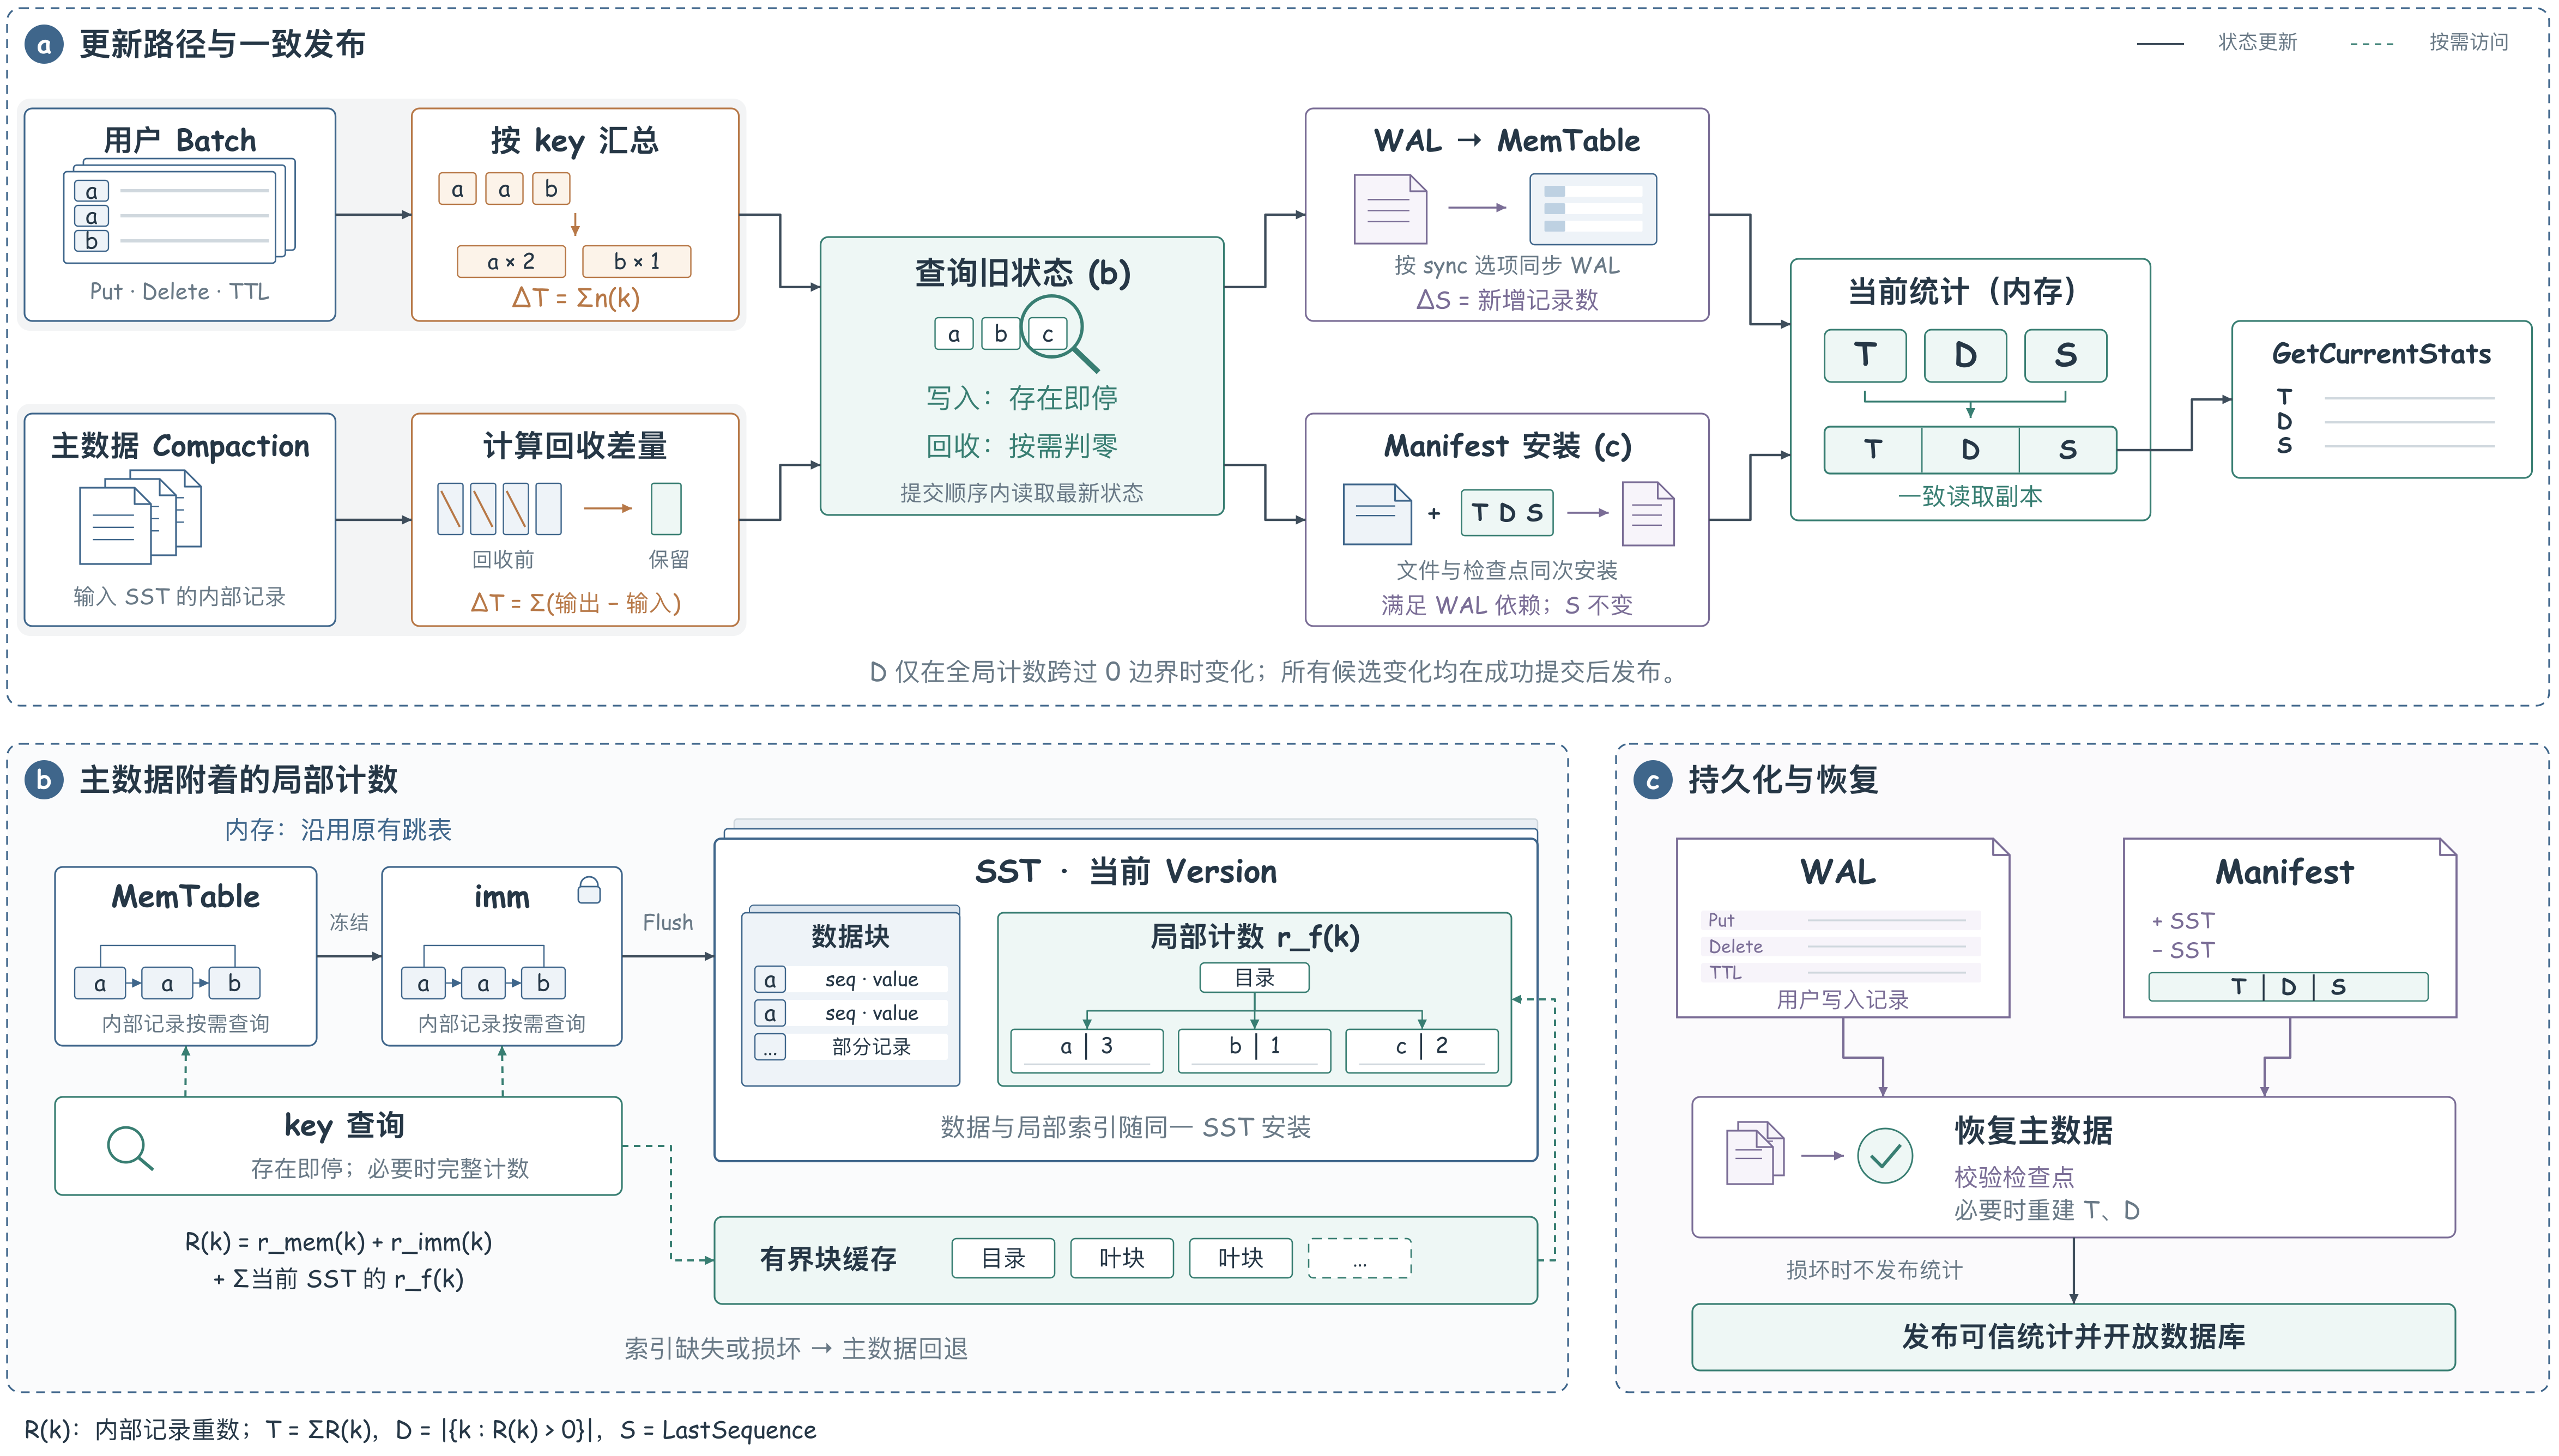
\includegraphics[width=\textwidth]{figures/metadata-overview-updated.png}
\caption{主数据附着式统计与当前状态查询总览（作者提供）。（a）更新路径与一致发布；（b）主数据附着的局部计数；（c）持久化与恢复。$T$、$D$、$S$ 分别为记录数、去重键数和发布序列号。写入按需判断键是否存在，回收按需精确计数。（c）为正常恢复主线；受限只读分支见第 4.3 节，图中损坏保护不涵盖所有畸形 WAL 批次。}
\label{fig:metadata-overview}
\end{figure*}
图~\ref{fig:metadata-overview} 展示统计信息如何附着在主数据结构并随提交发布。WAL 对应写入持久化，MANIFEST 对应文件版本安装，并非每次写入都修改 MANIFEST。

\subsection*{3.1 方案比较与最终取舍}
统计查询若每次扫描所有内部记录，容易实现精确口径，但代价随数据量增长；仅记录“当前可读键数”则不符合实验要求。我们维护全局记录数和去重键数，并在写入及回收时更新。


\begin{table}[htbp]
\centering
\small
\setlength{\tabcolsep}{3pt}
\renewcommand{\arraystretch}{1.25}
\caption{统计维护方案比较}
\label{tab:report-2}
\begin{tabularx}{\columnwidth}{@{}>{\hsize=0.78000\hsize\linewidth=\hsize\raggedright\arraybackslash}X>{\hsize=0.87000\hsize\linewidth=\hsize\raggedright\arraybackslash}X>{\hsize=1.35000\hsize\linewidth=\hsize\raggedright\arraybackslash}X@{}}
\toprule
\textbf{方案} & \textbf{优点} & \textbf{主要代价} \\
\midrule
每次全量扫描 & 口径直接 & 查询成本随规模增长 \\
全量内存键计数 & 按键更新方便 & 内存随不同键数增长 \\
主数据计数与全局标量 & 复用内部记录；查询快 & 写入需判断键是否已存在；合并需精确差分 \\
\bottomrule
\end{tabularx}
\end{table}

当前前台路径以主数据物理记录为依据：普通写入只需判断用户键是否已经存在，命中后立即停止；需要精确记录数的回收路径则查询局部计数索引或回退扫描。新增索引附着在每个 SST 中，不是独立辅助 LSM。MetadataIndex 仍被批次溢出、合并差分和重建的临时表读写及缓存复用；类中保留的辅助 LSM 代码不代表当前数据库仍采用该方案。Recover 明确拒绝带旧辅助元数据检查点、文件或提交记录的数据库，返回 NotSupported；这与缺少可选局部索引的旧 SST 可回退读取是两种不同的兼容边界。

\subsection*{3.2 写入提交与批次原子性}
WriteInternal 首先验证外部批次，并通过写队列串行确定提交组及序列号。对于每个不同用户键，检查提交前是否存在物理记录；记录总数增加批次内操作数，仅当原计数为零时增加去重键数。相同键在一个批次出现多次，只增加一次去重键数。设提交组含 $n$ 条操作，$K$ 为组内原始字节去重后的键集合，$R(k)$ 为提交前的物理记录数，则
\[
 T'=T+n,\qquad D'=D+\sum_{k\in K}\mathbf{1}_{R(k)=0}.
\]
该规则同时适用于普通值、TTL 值和删除标记。大批次键聚合超过工作区阈值时写入临时有序段并归并，避免必须在内存中保留整个批次的键集合。

实现先用已知最大键边界排除新键；写入键过滤器仅在默认字节序比较器下启用，且只覆盖启用时最大键边界之后的键。边界以内或自定义比较器路径不能直接套用过滤器的缺键结论。其余键由 \seqsplit{HasPrimaryRecordsForKey} 依次检查 MemTable、imm 和所有可能包含该键的 SST，任一来源命中即可停止，不再为普通写入累加完整记录数。失败写入留下的额外过滤标记最多增加查找次数，不得把已有键判为不存在。

WAL 追加及按需 Sync 成功后，批次插入 MemTable。重新持有状态锁后，再发布计数和最新序列号。失败路径不发布成功统计；Sync 失败会记录后台错误，阻止后续写入继续建立在不确定的持久化状态上。

为降低短时间写队列等待的切换成本，满足非同步写、可用 CPU 数和后台压力等条件时，少量等待线程可先短暂自旋；未获得执行机会时仍通过条件变量等待。组批时同步识别可信单条 Put 组，以减少后续重复遍历。该优化不改变批次提交与统计发布语义。

\subsection*{3.3 统计查询的快速路径}
常见计数范围内，将 total\_entries、distinct\_keys 和 seq 分别用 21、19、23 位编码进一个 64 位原子值，最高位标识回退。三个字段各自的上限分别为 $2^{21}-1$、$2^{19}-1$ 和 $2^{23}-1$。一次原子读取即可获得完整统计，不需要扫描数据或依次读取三个独立字段。

任一字段超过其对应的紧凑快照上限时，改用版本号保护的宽统计快照：$T$、$D$ 各占 32 位并打包，$S$ 单独保存在 64 位原子变量中。读者要求前后版本号相同且为偶数，并通过 acquire/release 屏障配合载荷读写；版本变化时重试。若 $T$ 或 $D$ 超过 $2^{32}-1$，或发布快照不可用，则进入加锁路径。因而“序列号超过 23 位”和“计数超过 32 位”触发的是不同层级的回退。

紧凑快照使常见范围内的查询无需获取数据库状态锁；超出范围时仍需经过宽快照校验或锁内读取。空指针参数返回 InvalidArgument；重建期间的查询等待或回退，避免读到未完成统计。

\begin{table}[!htbp]
\centering
\caption{紧凑统计快照的读取}
\label{tab:code-stats}
\setlength{\tabcolsep}{3pt}
\renewcommand{\arraystretch}{1.05}
\begin{tabularx}{\columnwidth}{@{}r>{\ttfamily\fontsize{7.5}{9.5}\selectfont\raggedright\arraybackslash}X@{}}
\toprule
{\small 行号} & {\normalfont\small 执行语句} \\
\midrule
1 & const uint64\_t compact\_snapshot = \\
2 & \hspace*{1.8em}published\_stats\_compact\_snapshot\_.load( \\
3 & \hspace*{3.6em}std::memory\_order\_relaxed); \\
4 & if ((compact\_snapshot \& kCompactStatsFallback) == 0) \{ \\
5 & \hspace*{0.9em}stats->total\_entries = \\
6 & \hspace*{2.7em}compact\_snapshot \& kCompactStatsTotalMask; \\
7 & \hspace*{0.9em}stats->distinct\_keys = \\
8 & \hspace*{2.7em}(compact\_snapshot >> kCompactStatsTotalBits) \\
9 & \hspace*{2.7em}\& kCompactStatsDistinctMask; \\
10 & \hspace*{0.9em}stats->seq = compact\_snapshot >> \\
11 & \hspace*{2.7em}(kCompactStatsTotalBits + \\
12 & \hspace*{3.6em}kCompactStatsDistinctBits); \\
13 & \hspace*{0.9em}return Status::OK(); \\
14 & \} \\
15 & return GetCurrentStatsWideSnapshot(stats); \\
\bottomrule
\end{tabularx}
\par\vspace{3pt}
\parbox{\columnwidth}{\footnotesize\raggedright\textbf{注：}摘自 \texttt{db/db\_impl.h} 的 \seqsplit{GetCurrentStatsSnapshot} 函数体，仅调整换行。三个字段来自同一原子值；置位回退标志时转入宽统计路径。}
\end{table}

表~\ref{tab:code-stats} 给出紧凑快照的读取代码；宽快照和锁内读取用于处理超出编码范围的情况。

\subsection*{3.4 Compaction 统计差分}
回收按用户键汇总输入、输出记录差分。total\_entries 随实际移除的内部记录减少；distinct\_keys 只有在当前数据库中该原始字节键的记录数从非零变为零时才减少。某个文件中不再出现该键，并不代表其他层或 MemTable 中也没有该键。


\begin{table}[htbp]
\centering
\small
\setlength{\tabcolsep}{3pt}
\renewcommand{\arraystretch}{1.25}
\caption{无回收时的统计示例}
\label{tab:report-3}
\begin{tabularx}{\columnwidth}{@{}>{\hsize=1.84000\hsize\linewidth=\hsize\raggedright\arraybackslash}X>{\hsize=0.72000\hsize\linewidth=\hsize\raggedright\arraybackslash}X>{\hsize=0.72000\hsize\linewidth=\hsize\raggedright\arraybackslash}X>{\hsize=0.72000\hsize\linewidth=\hsize\raggedright\arraybackslash}X@{}}
\toprule
\textbf{操作} & \textbf{记录数} & \textbf{键数} & \textbf{seq} \\
\midrule
空库 & 0 & 0 & 0 \\
Put(a,1) & 1 & 1 & 1 \\
Put(b,1) & 2 & 2 & 2 \\
Put(a,2) & 3 & 2 & 3 \\
Delete(b) & 4 & 2 & 4 \\
\bottomrule
\end{tabularx}
\end{table}

提交合并结果时，主 Version 和全局计数构成同一个发布状态。对于有记录变化的合并，代码协调写提交，等待正在进行的 WAL 组完成，再针对仍为当前的 Version 判断可能归零的键，并安装版本编辑。文件增删与新计数检查点写入同一个 VersionEdit；LogAndApply 成功后才更新内存标量并发布统计，合并本身不推进用户序列号。

例如，某键在合并前有 3 条记录，本次回收 3 条，期间前台又写入 1 条；提交时应按最新的 4 条减去 3 条，结果为 1 条，因此 $D$ 不变。上述提交边界避免使用过期计数覆盖并发写入，也防止 SST 构建或 MANIFEST 写入失败时提前扣除记录。若某键仍有输出记录，去重键数不变，无需再查该键；只有输出为零且发生记录减少时，普通合并才检查当前总数是否恰好等于移除量。已完整扫描且 Version 未变的底层路径，则检查输入之外是否仍有记录。两条路径都纳入并发写入，不能只用合并开始时的计数快照。没有统计差分的合并可跳过这一写提交阻塞阶段。

\subsection*{3.5 SST 逐键局部计数索引}
主数据 SST 的 metaindex 新增 \texttt{leveldb.local-counts.v1}，指向独立描述符块。描述符包含 LCI1 标识、树高、不同原始键数、物理记录总数与根块位置；它与文件级内部统计块分别校验；本次局部索引扩展不再改动 Footer、主记录编码与 MANIFEST 格式，但主数据统计方案本身已经增加了 MANIFEST 检查点字段。索引在刷盘、普通合并、底层重写和 RepairDB 的主数据输出中构建，通用 TableBuilder 和临时元数据表不启用。

计数树叶块存储“原始键 $\rightarrow$ fixed64 计数”，目录块存储“子块最大键 $\rightarrow$ BlockHandle”，均按字节序排序，目标块大小为 4 KiB，最多 32 层；4 KiB 是分块目标，单个长键可能使块超过该值，并非硬上限。默认字节序输入可流式聚合；自定义比较器下，按工作区预算生成带 CRC 的有序临时段，再最多 8 路归并。比较器判等但原始字节不同的键仍分别计数，旧版本、删除标记和未回收 TTL 记录均计入。

打开 SST 只读取小描述符，不预加载整棵计数树。局部计数块使用 metadata\_cache\_size 的一半作为缓存预算，剩余一半分给既有元数据缓存。缓存键包含全局唯一 Table 实例号和块偏移，避免重开或文件编号复用时命中旧内容；条目按实际保留容量计费，超出分片准入预算的大块直接读取。该预算约束缓存 charge，不代表整个进程的 RSS 上限。

旧 SST 缺失索引，或索引版本未知、CRC/结构校验失败时，禁用该 Table 实例的可选索引，并整体回退到验证主目录与数据块校验和的迭代器。零计数必须来自成功的索引查询或成功的主数据回退查询，不能把错误当成缺键。回退按用户比较器定位等价区间，再用原始字节确认目标键；存在性查询命中即停，精确计数遍历该键全部版本。主目录与实际读取的数据块校验失败必须向上传播，不能将这一按需检查描述为整库完整性证明。

局部索引属于单个 SST 的记录汇总：查询全局 $R(k)$ 时仍需合并所有相关来源，不能将局部键数直接相加。索引可选性描述的是已有 SST 的读取回退能力。构建新 SST 时，局部索引聚合、临时段或写块失败仍会使 TableBuilder 失败，不能安装该输出。文件级 \texttt{leveldb.internal-stats.v1} 摘要与逐键树分工不同：前者保存总记录数及 TTL 摘要，当前 LDS1 版本 2 不内嵌完整键计数表；后者加速逐键存在性和计数查询。GetCurrentStats 直接读取已发布标量，不逐次访问这棵树。原样 Flush 不改变全局计数，索引构建也不消耗用户序列号。

\section*{4 持久化恢复与完整 GC}
\subsection*{4.1 恢复路径}
TTL 截止时间属于记录本身，随 WAL、MemTable 和 SST 传递。恢复 WAL 时重放绝对截止时间；重新打开数据库不会为原记录延长有效期。恢复后的时间判断仍使用配置的 Env，便于用可控时钟验证边界。

统计恢复先检查 MANIFEST 的主数据检查点：要求检查点序列号不超过已记录的最新序列号，且总记录数不小于去重键数，并验证当前 SST 的内部统计块。严格模式还逐表读取数据块并校验；宽松模式不能因此宣称已验证全部主数据。WAL 重放遇到结束序列号超过检查点的非空批次时，会标记统计需要重建，而不是仅把日志操作数加到旧计数上。

RebuildMetadata 使用开启校验的内部迭代器扫描物理记录，包含删除标记、旧版本与过期值，同时重新计算 $T$ 与 $D$。默认字节序下按相邻键去重；自定义比较器下使用按原始字节排序的临时段与最多 8 路归并。只有完整扫描成功才替换全局计数并持久化检查点。该恢复成本与主数据规模有关，不能由“统计查询不扫描”推导为“重开也不扫描”。

文件损坏、读取错误和校验错误不应解释为“该文件记录数为零”。可选局部索引故障会回退主数据计数；检测到的主数据错误按所在恢复分支处理，精确统计重建失败时可按第 4.3 节进入受限只读状态。但该保护尚未覆盖所有畸形 WAL 批次。版本提交失败不能发布已完成回收的统计；已有故障测试覆盖部分 WAL、SST 和 MANIFEST 失败场景。

\subsection*{4.2 完整 GC 的可验证语义}
RunFullGC 返回 Status 和 GCResult。进入时捕获 entry\_sequence 与 entry\_time\_micros，以固定边界验证清理结果。Status::OK 只表示本次执行没有返回错误；只有 complete=true 才表示能证明该边界上的安全回收完成。


\begin{table}[htbp]
\centering
\small
\setlength{\tabcolsep}{3pt}
\renewcommand{\arraystretch}{1.25}
\caption{GCResult 的主要字段}
\label{tab:report-4}
\begin{tabularx}{\columnwidth}{@{}>{\hsize=0.98000\hsize\linewidth=\hsize\raggedright\arraybackslash}X>{\hsize=1.02000\hsize\linewidth=\hsize\raggedright\arraybackslash}X@{}}
\toprule
\textbf{字段} & \textbf{含义} \\
\midrule
complete & 本次可证明完成回收 \\
snapshots\_blocked & 观察到显式快照保护 \\
iterators\_blocked & 观察到用户迭代器占用 \\
\seqsplit{concurrent\_state\_changed} & 并发写入或版本变化影响完成证明 \\
\bottomrule
\end{tabularx}
\end{table}

实现先对入口 Version 的 SST 进行校验，再调用全范围整理；有资格声明完成时，还重新打开整理后 SST，避开可能未经校验进入共享缓存的块，再以内部迭代器检查重复版本、删除标记和入口时已过期记录。入口与结束阶段观测到快照、活动迭代器，或检测到并发写入及相关 Version 变化，都会阻止完成声明。另一项完整 GC 正在执行时，本次直接以 concurrent\_state\_changed 返回未完成；I/O、校验与后台错误通过 Status 返回。

complete 的参照时间是入口时间，不是函数返回时间。若记录在入口时仍有效、执行中才到期，本次可以保留它并返回 complete=true；此时当前 Get 已可返回 NotFound，物理统计仍包含该记录，下一次完整 GC 才会将其纳入到期回收范围。即使没有受保护视图，保守重写后仍留有重复版本也会使复核结果为未完成，不能将该接口理解为一次调用必然清空所有冗余记录。

\subsection*{4.3 损坏数据库的受限只读恢复}
系统对精确统计重建失败进行了明确处理：当 RebuildMetadata 返回 Corruption 且 paranoid\_checks=false 时，Open 可以成功返回一个受限只读对象，以便继续尝试读取完整记录。此时保留后台损坏状态，不发布部分统计，不启动正常后台维护；GetCurrentStats、写入和 RunFullGC 返回损坏错误，GC 不报告完成。读取也可能遇到损坏，不能把 Open 成功解释为数据完整。

若启用 paranoid\_checks，或重建失败属于其他错误，则不使用该宽松恢复分支。修复后需重新打开数据库才能恢复正常操作。这一边界同时写入公开 DB::Open 注释。CMake 的 Zstd 检测符号改为大小写正确的 ZSTD\_compress，使安装了对应库的环境能够正确检测并执行压缩相关测试。

\section*{5 正确性测试}
\subsection*{5.1 测试组织与验证目标}
正确性测试分为课程公开测试、项目新增定向测试和 LevelDB 原生回归三层。课程测试检查 TTL、统计接口及二者的联合行为；定向测试针对边界、并发、故障和恢复构造更细的场景；原生回归检查数据库原有功能、C 接口和 Env 接口。三层测试分别从接口契约、关键实现路径和兼容性验证系统。

\begin{table}[htbp]
\centering\small
\setlength{\tabcolsep}{4pt}
\renewcommand{\arraystretch}{1.2}
\caption{正确性测试的分层与检查内容}
\label{tab:correctness-scope}
\begin{tabularx}{\columnwidth}{@{}lY@{}}
\toprule
测试层次 & 主要检查内容 \\
\midrule
课程 TTL 测试 & TTL 接口、到期读写、快照及迭代器视图 \\
课程统计测试 & 内部记录计数、不同键数、序列号及重开恢复 \\
课程联合测试 & 混合覆盖、批次、快照、回收、重开和并发统计 \\
新增定向测试 & 边界时间、二进制键、局部索引、故障注入和随机模型 \\
原生兼容回归 & 原生数据库行为、C API 和 Env 接口 \\
\bottomrule
\end{tabularx}
\end{table}

\subsection*{5.2 课程公开测试}
课程公开 benchmark 包括两项 TTL 专项、两项统计专项和六项联合正确性场景；仓库还提供课程基础测试程序及项目新增的定向测试。TTL 专项检查过期读取及固定视图；统计专项检查计数契约和重开后的统计。六项联合测试分别覆盖基本接口、覆盖与删除、快照和迭代器、重开恢复、过期回收以及并发写入时的统计查询。

联合测试将普通写入、TTL 写入与删除组合起来，验证记录到期后读取结果发生变化，而统计只有在记录被实际回收并成功安装后才减少；同时检查回收不推进用户序列号。重开场景分别检查 WAL 和 SST 路径，确认截止时间与统计结果得到恢复。并发场景持续读取统计，检查同一批次不会只发布部分结果。

\subsection*{5.3 新增定向测试}
在公开测试基础上，项目围绕以下关键问题补充测试。

\begin{enumerate}
\item \textbf{时间边界与读取视图。}检查零 TTL、恰好到期、截止时间溢出、旧值屏蔽，以及快照和双向迭代器在到期与回收前后的读取。混合批次示例中，写入后统计为 $(6,3,6)$；释放视图并完成 GC 后，只保留永久值，统计变为 $(1,1,6)$，重开后保持一致。
\item \textbf{统计更新与并发。}测试同键跨 MemTable、imm 和 SST 的计数、批次内重复键，以及合并期间同键写入；检查 $T$、$D$、$S$ 按整体发布。另通过随机操作序列与独立模型对照，检查读取结果和静止状态下的物理记录统计。
\item \textbf{局部索引与特殊键。}测试 SST 局部计数索引的构建、查询、多层结构、缓存淘汰与损坏回退，并覆盖空键、二进制键和自定义比较器下的原始字节判等。可选索引不可用时从主数据计数，主数据读取失败时返回错误。
\item \textbf{回收、故障与恢复。}检查底层重写、部分范围回收、摘要缺失或损坏、显式快照保护和完整 GC 的结果；注入 WAL、SST 同步及 MANIFEST 写入失败，并在进程终止后检查恢复，确认失败安装不会提前发布回收减量。
\end{enumerate}
上述具体数值属于测试代码中的断言，用于说明测试内容；实际通过情况以对应运行记录为准。

\subsection*{5.4 测试结果}
三组对照实验共完成 372 次课程场景运行，全部通过；该总数包含正确性与性能场景，且课程初始实现只运行其支持的场景。当前实现的固定版本原生回归连续三轮均为 211/211 通过，C 接口回归三轮通过，Env 回归三轮均为 7/7 通过。[1] 这组结果验证了运行记录覆盖的公开场景和兼容性回归；项目新增定向测试的断言见第 5.3 节，不以该总数代替其独立执行结果。


\section*{6 性能测试与结果分析}
\subsection*{6.1 测试方案与评价指标}
性能测试采用课程公开 benchmark，同时考察普通读写、TTL 和元数据统计。对比包括课程初始实现、加入 TTL 与元数据统计后的早期实现和当前实现。课程初始实现不支持 TTL 与统计接口，因此只参加共有普通性能场景的比较；专项场景比较后两种实现。[1]

实验在同一台 Ubuntu 20.04（Linux x86\_64）机器上进行，处理器为 Intel Xeon Platinum 8375C，主频 2.90 GHz，系统可见 4 核、8 线程；物理内存约 15.35 GiB（MemTotal 为 16,097,684 KiB），C++ 编译器为 GCC/G++ 9.3.0。各实现采用独立 Release 构建，启用 Snappy 和 Zstd。测试规模为 1 万和 10 万键，适用场景使用 1 或 8 个线程，TTL 场景覆盖 0\%、50\% 和 100\% 过期比例，值大小为 256 字节。各配置运行三次，使用相同参数和对应随机种子，交替运行各实现，表中给出三次吞吐量的中位数。共完成 372 次场景运行，覆盖 80 个性能阶段与配置。[1]

课程 benchmark 的性能项包括普通写入、并发写入、命中与未命中读取、扫描和数据库重开；TTL 专项测量 TTL 写入、混合读取与完整回收；统计专项测量统计查询和写入期间的查询；联合场景测量 TTL 写入与统计查询、不同过期比例下的联合回收。吞吐量包含测试驱动的工作，GC 阶段使用配置键数除以阶段耗时，表示阶段处理率。

\subsection*{6.2 普通读写与恢复性能}
表~\ref{tab:perf-common} 展示 10 万键场景下的主要结果。当前实现的单线程写入、八线程并发写入、命中读取和数据库重开吞吐均高于两个对照实现；扫描吞吐与课程初始实现接近。重开指标的单位为次/s，其余为操作/s。[1]

\begin{table}[htbp]
\centering\small
\setlength{\tabcolsep}{4pt}
\renewcommand{\arraystretch}{1.2}
\caption{10 万键普通性能场景的吞吐量中位数}
\label{tab:perf-common}
\begin{tabularx}{\columnwidth}{@{}Yrrr@{}}
\toprule
场景 & 课程初始 & 附着初期 & 当前实现 \\
\midrule
单线程写入 & 101,562 & 63,997 & 482,424 \\
八线程并发写入 & 66,632 & 47,851 & 163,066 \\
命中读取 & 689,408 & 643,243 & 909,688 \\
扫描 & 2,593,240 & 2,329,820 & 2,579,180 \\
数据库重开（次/s） & 112.67 & 66.13 & 252.79 \\
\bottomrule
\end{tabularx}
\end{table}

当前实现的普通单线程写入较课程初始实现提高 375.00\%，八线程并发写入提高 144.73\%；重开吞吐提高 124.38\%。这些结果反映不同实现整体的表现，不能将差异单独归因于某一项优化。

\subsection*{6.3 TTL 与统计专项性能}
表~\ref{tab:perf-special} 比较具备 TTL 和统计功能的两个实现。10 万键 TTL 写入吞吐由 63,324 提高到 470,104 次/s；八线程写入期间统计查询由 7,566,200 提高到 19,438,400 次/s。TTL 完整 GC 和 50\% 过期比例下的联合 GC 阶段处理率也有明显提高。[1]

\begin{table}[htbp]
\centering\small
\setlength{\tabcolsep}{4pt}
\renewcommand{\arraystretch}{1.2}
\caption{10 万键 TTL 与统计场景的吞吐量中位数}
\label{tab:perf-special}
\begin{tabularx}{\columnwidth}{@{}Yrrr@{}}
\toprule
场景 & 附着初期 & 当前实现 & 变化 \\
\midrule
TTL 写入 & 63,324 & 470,104 & +642.38\% \\
写入期间统计查询（8 线程） & 7,566,200 & 19,438,400 & +156.91\% \\
TTL 完整 GC & 279,024 & 4,321,590 & +1448.82\% \\
联合 GC（50\% 过期） & 354,877 & 1,916,900 & +440.16\% \\
\bottomrule
\end{tabularx}
\end{table}

TTL 完整 GC 和联合 GC 的数字是基于配置键数计算的阶段处理率，不表示磁盘实际每秒执行的 I/O 次数。统计查询与写入的并发测试分别记录两类操作：10 万键、8 线程下，当前实现有查询时写入为 156,497 次/s，无查询时为 161,767 次/s，按两者中位数计算下降约 3.26\%。这一差异用于衡量该配置下的查询干扰，仍可能受三轮测量波动影响。

\subsection*{6.4 结果分析与补充测试}
性能并非在所有配置下都提高：1 万键、8 线程且并发查询统计时，写入吞吐从 54,733.60 降至 50,914.00 次/s，下降 6.98\%；1 万键重开和扫描分别比课程初始实现低 4.34\% 和 2.02\%。这些差异基于三次中位数，仍需通过更多重复实验观察波动。[1]

表~\ref{tab:result-variation} 给出当前实现三个代表性配置的三轮最小值、中位数和最大值，用以展示实验波动。全部结果见附录 C。

\begin{table}[htbp]
\centering\small
\setlength{\tabcolsep}{3pt}
\renewcommand{\arraystretch}{1.2}
\caption{10 万键代表场景的三轮吞吐量范围（次/s）}
\label{tab:result-variation}
\begin{tabularx}{\columnwidth}{@{}Yrrr@{}}
\toprule
场景 & 最小值 & 中位数 & 最大值 \\
\midrule
单线程写入 & 481,723 & 482,424 & 493,231 \\
八线程并发写入 & 162,561 & 163,066 & 164,551 \\
TTL 完整 GC & 4,082,800 & 4,321,590 & 4,427,210 \\
\bottomrule
\end{tabularx}
\end{table}

资源方面，10 万键单线程普通写入的峰值 RSS 中位数分别为课程初始实现 30,540 KiB、附着初期 30,732 KiB、当前实现 41,404 KiB。RSS 包含测试驱动、数据模型和缓存，反映进程整体内存而非数据库独占内存。[1]

除课程 benchmark 外，项目还提供针对局部计数索引的定向微基准，分别观察索引构建、文件空间和冷暖查询成本；已有记录表明，不同键数和版本密度组合下的索引空间与查询收益存在差异；由于两个因素同时变化，不能单独归因于版本密度。这些定向实验帮助分析成本来源，不能直接替代整库性能测试。后续可增加重复次数，并结合阶段耗时、缓存命中和 I/O 指标分析写入与回收中的具体开销。

\section*{7 实验问题与解决方法}
\subsection*{7.1 过期记录与统计口径冲突}
最容易混淆的是“用户读不到”和“物理记录不存在”。如果在 Get 判断到期时直接扣减统计，多个读线程可能重复扣减，时间流逝也会改变统计却没有对应版本提交。实现上，Get 和迭代器的过期过滤只影响读取可见性，不直接扣减物理统计；合并与底层重写仍按过期时间、快照和版本屏障判断能否删除。回收造成的统计减量与对应文件变更一起提交，安装成功后才发布。

\subsection*{7.2 范围回收与空输出}
最底层重写必须处理只清理部分键、边界文件同时包含范围内外记录，以及全部过期后无输出文件的情况。当前实现限定重写文件集合，按比较器保留范围外记录，并将输出文件编号初始化为 0，避免空输出时使用未初始化值。范围测试检查可见性、物理计数与不相交文件身份；空输出另经源码检查，上述测试不代表所有空输出分支均已覆盖。

\subsection*{7.3 并发与持久化失败}
合并准备期间，同一用户键可能被前台再次写入。如果按旧状态计算 distinct\_keys 的减量，就会把仍有新记录的键错误扣除。实现通过 BeginMetadataCommit 暂停新的写提交，并等待正在进行的 WAL 写入完成；只有本次合并不再输出的键，才需要查询当前主数据，核对全局物理计数是否从非零变为零。文件变更与统计检查点通过同一 VersionEdit 安装，成功后更新已发布统计。并发同键写入测试在 SST 同步处暂停合并，再插入新值，验证读取和物理统计仍一致。

文件创建成功不代表版本提交成功。当前 SST 同步或 MANIFEST 安装失败时，不发布这次失败安装的文件变更和统计减量；这不意味着回滚整个 GC 中此前已成功提交的步骤。错误的对外呈现依接口而异：RunFullGC 返回失败 Status 并将 complete 置为 false；返回 void 的 CompactRange 记录后台错误，不能直接向调用者返回 Status。故障注入分别覆盖普通合并和底层重写的 SST Sync、MANIFEST Append 失败，并检查发布状态与恢复行为；这些用例不构成对所有存储故障的完整覆盖。

\section*{8 实验总结}
本实验的主要收获是将可见性、物理保存状态和持久化提交分开建模：TTL 决定读取结果，当前 Version 决定统计范围，成功提交决定发布时机。三者的边界明确后，零 TTL、旧版本屏蔽、快照保护和回收计数才能形成一致的实现。

本实验完成了 TTL 与统计元数据的联合设计：写入保存绝对截止时间，读取按固定视图判定可见性，回收依据快照及版本边界过滤记录；统计则依据主数据记录，在写入和文件安装时更新，并通过检查点与重建恢复。课程场景和原生回归结果支持上述接口在已测试条件下的正确性。

性能对照显示，当前实现的部分普通写入、TTL 写入与回收场景吞吐有明显提升，同时也存在小规模并发写入下降和进程内存增加。后续应优先完善畸形 WAL 批次恢复和宽时间分布下的过期估计，补充故障测试与更多重复测量，再针对计数索引构建、冷块访问和回收过程开展性能分析。

\section*{附录 复现入口与证据索引}
\subsection*{A 构建和运行}
建议在 Linux 或 WSL2 的 Linux 文件系统中构建和测试，使用 CMake 3.22+、支持 C++17 的编译器及 Python 3.9+。复现本文实现应先取得远程仓库中的源码；以下点号表示该源码根目录。课程测试应在独立数据库目录运行，每次 benchmark 使用全新输出目录。


\begin{table}[!htbp]
\centering
\caption{构建与原生测试命令}
\label{tab:cmd-build}
\setlength{\tabcolsep}{3pt}
\renewcommand{\arraystretch}{1.05}
\begin{tabularx}{\columnwidth}{@{}r>{\ttfamily\fontsize{7.5}{9.5}\selectfont\raggedright\arraybackslash}X@{}}
\toprule
{\small 行号} & {\normalfont\small 执行语句} \\
\midrule
1 & cmake -S . -B build \textbackslash{} \\
2 & \hspace*{0.9em}-DCMAKE\_BUILD\_TYPE=Debug \textbackslash{} \\
3 & \hspace*{0.9em}-DLEVELDB\_BUILD\_TESTS=ON \textbackslash{} \\
4 & \hspace*{0.9em}-DLEVELDB\_BUILD\_BENCHMARKS=OFF \\
5 & cmake --build build -j2 \\
6 & ctest --test-dir build --output-on-failure \\
7 & ./build/ttl\_test \\
8 & ./build/metadata\_test \\
\bottomrule
\end{tabularx}
\par\vspace{3pt}
\parbox{\columnwidth}{\footnotesize\raggedright\textbf{注：}在远程仓库根目录的 Linux shell 中执行，反斜杠表示续行。Debug 构建启用测试并关闭基准程序；\texttt{ctest} 在失败时输出日志。}
\end{table}
表~\ref{tab:cmd-build} 给出构建与测试入口。第 6 行仅运行已注册的 CTest 测试；课程独立程序未注册到 CTest，故第 7、8 行须单独执行。专项测试可通过 leveldb\_tests 的 gtest\_filter 选择 TTLMetadataTest。第 5.4 节列出不同批次的实际执行结果。压缩库缺失会使部分原生测试跳过，应检查跳过原因，而非只看 CTest 的成功状态。


\begin{table}[!htbp]
\centering
\caption{联合基准测试命令}
\label{tab:cmd-benchmark}
\setlength{\tabcolsep}{3pt}
\renewcommand{\arraystretch}{1.05}
\begin{tabularx}{\columnwidth}{@{}r>{\ttfamily\fontsize{7.5}{9.5}\selectfont\raggedright\arraybackslash}X@{}}
\toprule
{\small 行号} & {\normalfont\small 执行语句} \\
\midrule
1 & python3 benchmark/runner.py \textbackslash{} \\
2 & \hspace*{0.9em}--kind combined --source . \textbackslash{} \\
3 & \hspace*{0.9em}--output /tmp/leveldb-report-run-001 \textbackslash{} \\
4 & \hspace*{0.9em}--profile standard --matrix \textbackslash{} \\
5 & \hspace*{0.9em}--repeat 3 --jobs 2 \\
\bottomrule
\end{tabularx}
\par\vspace{3pt}
\parbox{\columnwidth}{\footnotesize\raggedright\textbf{注：}从仓库根目录运行；输出目录为示例路径，每次应换用全新目录。此处为当前源码的 3 次重复运行示例。正文三组对照需要分别准备对应源码并按相同参数运行；实验口径与原始数据见 [1]。}
\end{table}
联合基准测试入口见表~\ref{tab:cmd-benchmark}。检查 summary.json 的 full\_suite、status 与 regression，并结合 aggregate.json、metrics.csv 查看重复结果。各场景的测试配置和测量结果见 [1]。

\subsection*{B 实验结果文件}
\begingroup\raggedright
{\small 以下文件位于仓库的 \seqsplit{doc/THREE\_VERSION\_BENCHMARK\_20261105/} 目录。[1]\par}

{\small \texttt{REPORT.md}：实验方法、测试结果和性能分析。\par}
{\small \texttt{metrics-raw.csv}：各轮场景的原始性能数据。\par}
{\small \texttt{metrics-median.csv}：各配置的中位数与波动范围。\par}
{\small \texttt{peak-rss.csv}：各场景的进程峰值内存数据。\par}
{\small \texttt{benchmark-summary.json}：场景运行汇总。\par}
{\small \texttt{regressions-summary.json}、\seqsplit{regression-followup-summary.json}：原生回归及补充验证结果。\par}
{\small \texttt{run-manifest.json}：实验配置和运行记录。\par}

\endgroup
\clearpage
\onecolumn
\section*{附录 C 三组实验数据中位数}
本附录汇总课程初始实现、功能加入后的早期实现和当前实现的全部已记录中位数。每项配置重复三次；数据来自附录 B 的 \texttt{metrics-median.csv} 与 \texttt{peak-rss.csv}。初始实现不支持 TTL 和统计接口，因此相应场景没有数据。各指标分别取三次运行的中位数，不保证对应同一次运行。

表中 $N$ 为配置键数或操作规模，线程数和过期率为运行参数；不适用过期率的场景仍保留运行器记录的参数。吞吐量单位为操作/s，重开场景为次/s；耗时单位为 s，延迟单位为 $\mu$s。GC 吞吐量按配置键数除以阶段耗时计算。写入量为测量阶段的追加字节数，目录大小为排空后的数据库目录字节数，均非物理设备 I/O。峰值 RSS 的单位为 KiB，包含测试驱动和缓存。表中按原始数据保留数值精度；重复运行的最小值和最大值见附录 B 数据文件。

\subsection*{C.1 性能场景与阶段编号}
\begin{center}\small
\begin{tabular}{@{}lll@{}}
\toprule
编号 & 场景 & 阶段 \\
\midrule
P01 & \texttt{perf\_combined\_gc} & \texttt{ttl\_gc\_with\_statistics} \\
P02 & \texttt{perf\_combined\_stats\_under\_write} & \texttt{stats\_under\_ttl\_write} \\
P03 & \texttt{perf\_combined\_stats\_under\_write} & \texttt{ttl\_put\_with\_stats\_queries} \\
P04 & \texttt{perf\_combined\_stats\_under\_write} & \texttt{ttl\_put\_without\_stats\_queries} \\
P05 & \texttt{perf\_concurrent} & \texttt{parallel\_put} \\
P06 & \texttt{perf\_read} & \texttt{get\_hit} \\
P07 & \texttt{perf\_read} & \texttt{get\_miss} \\
P08 & \texttt{perf\_reopen} & \texttt{open} \\
P09 & \texttt{perf\_scan} & \texttt{scan} \\
P10 & \texttt{perf\_stats} & \texttt{stats\_query} \\
P11 & \texttt{perf\_stats\_under\_write} & \texttt{put\_with\_stats\_queries} \\
P12 & \texttt{perf\_stats\_under\_write} & \texttt{put\_without\_stats\_queries} \\
P13 & \texttt{perf\_stats\_under\_write} & \texttt{stats\_under\_write} \\
P14 & \texttt{perf\_ttl\_gc} & \texttt{ttl\_full\_gc} \\
P15 & \texttt{perf\_ttl\_mixed} & \texttt{ttl\_mixed\_get} \\
P16 & \texttt{perf\_ttl\_write} & \texttt{ttl\_put} \\
P17 & \texttt{perf\_write} & \texttt{put} \\
\bottomrule
\end{tabular}
\end{center}
\subsection*{C.2 性能指标中位数}
\begingroup\scriptsize
\setlength{\tabcolsep}{3pt}
\begin{longtable}{@{}lrrrlrrrrrrr@{}}
\caption{各性能阶段的三次运行中位数}\\
\toprule
编号 & $N$ & 线程 & 过期\% & 实现 & 吞吐量 & 耗时 & p50 & p95 & p99 & 写入字节 & 目录字节 \\
\midrule
\endfirsthead
\toprule
编号 & $N$ & 线程 & 过期\% & 实现 & 吞吐量 & 耗时 & p50 & p95 & p99 & 写入字节 & 目录字节 \\
\midrule
\endhead
\bottomrule
\endfoot
P01 & 10000 & 1 & 0 & 早期 & 316939 & 0.0315518 & 31551.1 & 31551.1 & 31551.1 & 2814090 & 2839675 \\
P01 & 10000 & 1 & 0 & 当前 & 659388 & 0.0151656 & 15159.8 & 15159.8 & 15159.8 & 3110822 & 3127143 \\
P01 & 10000 & 1 & 50 & 早期 & 274626 & 0.0364132 & 36412.4 & 36412.4 & 36412.4 & 1521762 & 1432844 \\
P01 & 10000 & 1 & 50 & 当前 & 763176 & 0.0131031 & 13102.5 & 13102.5 & 13102.5 & 1555602 & 1571924 \\
P01 & 10000 & 1 & 100 & 早期 & 278003 & 0.0359709 & 35970.2 & 35970.2 & 35970.2 & 229200 & 25229 \\
P01 & 10000 & 1 & 100 & 当前 & 1877690 & 0.00532569 & 5325.02 & 5325.02 & 5325.02 & 30 & 16353 \\
P01 & 100000 & 1 & 0 & 早期 & 461482 & 0.216693 & 216692 & 216692 & 216692 & 28141412 & 28297111 \\
P01 & 100000 & 1 & 0 & 当前 & 1201120 & 0.0832554 & 83254.4 & 83254.4 & 83254.4 & 31106623 & 31182999 \\
P01 & 100000 & 1 & 50 & 早期 & 354877 & 0.281788 & 281782 & 281782 & 281782 & 15217588 & 14228396 \\
P01 & 100000 & 1 & 50 & 当前 & 1916900 & 0.0521675 & 52166.6 & 52166.6 & 52166.6 & 15553418 & 15629795 \\
P01 & 100000 & 1 & 100 & 早期 & 280561 & 0.356429 & 356428 & 356428 & 356428 & 2294330 & 158823 \\
P01 & 100000 & 1 & 100 & 当前 & 4299590 & 0.023258 & 23251.1 & 23251.1 & 23251.1 & 129 & 76507 \\
P02 & 10000 & 1 & 0 & 早期 & 10092200 & 0.14686 & 0.051 & 0.054 & 0.087 & 5769235 & 5658527 \\
P02 & 10000 & 1 & 0 & 当前 & 19791900 & 0.0208093 & 0.03 & 0.031 & 0.098 & 3030567 & 6166358 \\
P02 & 10000 & 1 & 50 & 早期 & 9928650 & 0.147807 & 0.051 & 0.06 & 0.091 & 5769235 & 5658528 \\
P02 & 10000 & 1 & 50 & 当前 & 19383400 & 0.0211321 & 0.03 & 0.031 & 0.078 & 3030567 & 6166359 \\
P02 & 10000 & 1 & 100 & 早期 & 10232200 & 0.146924 & 0.051 & 0.053 & 0.088 & 5769235 & 5658529 \\
P02 & 10000 & 1 & 100 & 当前 & 19741600 & 0.021061 & 0.03 & 0.031 & 0.087 & 3030567 & 6166360 \\
P02 & 10000 & 8 & 0 & 早期 & 6999120 & 0.176534 & 0.051 & 0.057 & 0.09 & 8022482 & 5655015 \\
P02 & 10000 & 8 & 0 & 当前 & 17213900 & 0.0627564 & 0.032 & 0.048 & 0.076 & 2886911 & 6026016 \\
P02 & 10000 & 8 & 50 & 早期 & 7221120 & 0.176487 & 0.051 & 0.056 & 0.088 & 8022475 & 5654509 \\
P02 & 10000 & 8 & 50 & 当前 & 17395500 & 0.0625325 & 0.032 & 0.047 & 0.076 & 2887815 & 6026864 \\
P02 & 10000 & 8 & 100 & 早期 & 7475910 & 0.183521 & 0.051 & 0.053 & 0.085 & 8027585 & 5655170 \\
P02 & 10000 & 8 & 100 & 当前 & 16324700 & 0.0642011 & 0.032 & 0.047 & 0.073 & 2887634 & 6027063 \\
P02 & 100000 & 1 & 0 & 早期 & 7626500 & 1.63628 & 0.051 & 0.053 & 0.095 & 58377475 & 56445182 \\
P02 & 100000 & 1 & 0 & 当前 & 19310200 & 0.217366 & 0.03 & 0.032 & 0.073 & 61120076 & 62539100 \\
P02 & 100000 & 1 & 50 & 早期 & 7900800 & 1.64452 & 0.051 & 0.052 & 0.063 & 58377475 & 56452036 \\
P02 & 100000 & 1 & 50 & 当前 & 19517700 & 0.227455 & 0.03 & 0.031 & 0.082 & 61120076 & 62539101 \\
P02 & 100000 & 1 & 100 & 早期 & 7718790 & 1.6504 & 0.051 & 0.052 & 0.065 & 58377475 & 56453654 \\
P02 & 100000 & 1 & 100 & 当前 & 19061800 & 0.207368 & 0.03 & 0.045 & 0.079 & 61120076 & 62539102 \\
P02 & 100000 & 8 & 0 & 早期 & 7319470 & 2.22243 & 0.051 & 0.055 & 0.084 & 101630325 & 56436986 \\
P02 & 100000 & 8 & 0 & 当前 & 17088500 & 0.639124 & 0.032 & 0.049 & 0.065 & 59713784 & 62522567 \\
P02 & 100000 & 8 & 50 & 早期 & 7429520 & 2.25246 & 0.051 & 0.054 & 0.087 & 107092190 & 56439913 \\
P02 & 100000 & 8 & 50 & 当前 & 17203800 & 0.639486 & 0.032 & 0.047 & 0.061 & 59715739 & 62522579 \\
P02 & 100000 & 8 & 100 & 早期 & 7339910 & 2.20679 & 0.051 & 0.053 & 0.09 & 102458095 & 56447376 \\
P02 & 100000 & 8 & 100 & 当前 & 17320100 & 0.645695 & 0.032 & 0.047 & 0.071 & 59717591 & 62523199 \\
P03 & 10000 & 1 & 0 & 早期 & 68074.9 & 0.146897 & 0 & 0 & 0 & 5769162 & 5658527 \\
P03 & 10000 & 1 & 0 & 当前 & 479689 & 0.0208468 & 0 & 0 & 0 & 3030567 & 6166358 \\
P03 & 10000 & 1 & 50 & 早期 & 67637 & 0.147848 & 0 & 0 & 0 & 5769162 & 5658528 \\
P03 & 10000 & 1 & 50 & 当前 & 472172 & 0.0211787 & 0 & 0 & 0 & 3030567 & 6166359 \\
P03 & 10000 & 1 & 100 & 早期 & 68040.4 & 0.146971 & 0 & 0 & 0 & 5769162 & 5658529 \\
P03 & 10000 & 1 & 100 & 当前 & 473818 & 0.0211051 & 0 & 0 & 0 & 3030567 & 6166360 \\
P03 & 10000 & 8 & 0 & 早期 & 56568.5 & 0.176777 & 0 & 0 & 0 & 7227673 & 5655015 \\
P03 & 10000 & 8 & 0 & 当前 & 158870 & 0.0629446 & 0 & 0 & 0 & 2890225 & 6026016 \\
P03 & 10000 & 8 & 50 & 早期 & 56611.3 & 0.176643 & 0 & 0 & 0 & 7403425 & 5654509 \\
P03 & 10000 & 8 & 50 & 当前 & 159445 & 0.0627176 & 0 & 0 & 0 & 2891072 & 6026864 \\
P03 & 10000 & 8 & 100 & 早期 & 54436.2 & 0.183701 & 0 & 0 & 0 & 7801984 & 5655170 \\
P03 & 10000 & 8 & 100 & 当前 & 155107 & 0.0644718 & 0 & 0 & 0 & 2891270 & 6027063 \\
P03 & 100000 & 1 & 0 & 早期 & 61112.7 & 1.63632 & 0 & 0 & 0 & 58377399 & 56445182 \\
P03 & 100000 & 1 & 0 & 当前 & 459967 & 0.217407 & 0 & 0 & 0 & 56658526 & 62539100 \\
P03 & 100000 & 1 & 50 & 早期 & 60805.9 & 1.64458 & 0 & 0 & 0 & 58377399 & 56452036 \\
P03 & 100000 & 1 & 50 & 当前 & 439557 & 0.227502 & 0 & 0 & 0 & 56931593 & 62539101 \\
P03 & 100000 & 1 & 100 & 早期 & 60589.6 & 1.65045 & 0 & 0 & 0 & 58377399 & 56453654 \\
P03 & 100000 & 1 & 100 & 当前 & 482117 & 0.207419 & 0 & 0 & 0 & 56869298 & 62539102 \\
P03 & 100000 & 8 & 0 & 早期 & 44992.2 & 2.22261 & 0 & 0 & 0 & 100274520 & 56436986 \\
P03 & 100000 & 8 & 0 & 当前 & 156403 & 0.639372 & 0 & 0 & 0 & 57153850 & 62522567 \\
P03 & 100000 & 8 & 50 & 早期 & 44390.8 & 2.25272 & 0 & 0 & 0 & 105958144 & 56439913 \\
P03 & 100000 & 8 & 50 & 当前 & 156330 & 0.639671 & 0 & 0 & 0 & 57295053 & 62522579 \\
P03 & 100000 & 8 & 100 & 早期 & 45310.7 & 2.20698 & 0 & 0 & 0 & 101558312 & 56447376 \\
P03 & 100000 & 8 & 100 & 当前 & 154828 & 0.645878 & 0 & 0 & 0 & 56988546 & 62523199 \\
P04 & 10000 & 1 & 0 & 早期 & 68798.4 & 0.145352 & 0 & 0 & 0 & 5769162 & 5658527 \\
P04 & 10000 & 1 & 0 & 当前 & 484948 & 0.0206208 & 0 & 0 & 0 & 3030567 & 6166358 \\
P04 & 10000 & 1 & 50 & 早期 & 69049.7 & 0.144823 & 0 & 0 & 0 & 5769162 & 5658528 \\
P04 & 10000 & 1 & 50 & 当前 & 476541 & 0.0209845 & 0 & 0 & 0 & 3030567 & 6166359 \\
P04 & 10000 & 1 & 100 & 早期 & 69249.6 & 0.144405 & 0 & 0 & 0 & 5769162 & 5658529 \\
P04 & 10000 & 1 & 100 & 当前 & 483207 & 0.020695 & 0 & 0 & 0 & 3030567 & 6166360 \\
P04 & 10000 & 8 & 0 & 早期 & 57052.3 & 0.175278 & 0 & 0 & 0 & 7080622 & 5654895 \\
P04 & 10000 & 8 & 0 & 当前 & 163399 & 0.0612 & 0 & 0 & 0 & 2889256 & 6025047 \\
P04 & 10000 & 8 & 50 & 早期 & 57412.4 & 0.174179 & 0 & 0 & 0 & 7137661 & 5654345 \\
P04 & 10000 & 8 & 50 & 当前 & 164058 & 0.0609542 & 0 & 0 & 0 & 2889047 & 6024839 \\
P04 & 10000 & 8 & 100 & 早期 & 57440.3 & 0.174094 & 0 & 0 & 0 & 6802483 & 5654551 \\
P04 & 10000 & 8 & 100 & 当前 & 165081 & 0.0605764 & 0 & 0 & 0 & 2889294 & 6025087 \\
P04 & 100000 & 1 & 0 & 早期 & 62384.1 & 1.60297 & 0 & 0 & 0 & 58377399 & 56454653 \\
P04 & 100000 & 1 & 0 & 当前 & 466239 & 0.214482 & 0 & 0 & 0 & 56890063 & 62539100 \\
P04 & 100000 & 1 & 50 & 早期 & 62515.2 & 1.59961 & 0 & 0 & 0 & 58377399 & 56462585 \\
P04 & 100000 & 1 & 50 & 当前 & 440008 & 0.227269 & 0 & 0 & 0 & 56964470 & 62539101 \\
P04 & 100000 & 1 & 100 & 早期 & 62592.5 & 1.59764 & 0 & 0 & 0 & 58377399 & 56464896 \\
P04 & 100000 & 1 & 100 & 当前 & 495001 & 0.20202 & 0 & 0 & 0 & 56952062 & 62539102 \\
P04 & 100000 & 8 & 0 & 早期 & 45144.2 & 2.21512 & 0 & 0 & 0 & 99664689 & 56443733 \\
P04 & 100000 & 8 & 0 & 当前 & 162999 & 0.6135 & 0 & 0 & 0 & 57047595 & 62523039 \\
P04 & 100000 & 8 & 50 & 早期 & 45392.7 & 2.203 & 0 & 0 & 0 & 99038527 & 56433229 \\
P04 & 100000 & 8 & 50 & 当前 & 164066 & 0.60951 & 0 & 0 & 0 & 57045789 & 62521943 \\
P04 & 100000 & 8 & 100 & 早期 & 45594.3 & 2.19326 & 0 & 0 & 0 & 100818526 & 56445051 \\
P04 & 100000 & 8 & 100 & 当前 & 162541 & 0.615228 & 0 & 0 & 0 & 57024687 & 62522368 \\
P05 & 10000 & 1 & 50 & 初始 & 115213 & 0.0867961 & 0 & 0 & 0 & 5639813 & 2748356 \\
P05 & 10000 & 1 & 50 & 早期 & 69953.7 & 0.142952 & 0 & 0 & 0 & 5642345 & 2751735 \\
P05 & 10000 & 1 & 50 & 当前 & 501160 & 0.0199537 & 0 & 0 & 0 & 2950595 & 2959127 \\
P05 & 10000 & 8 & 50 & 初始 & 87837.3 & 0.113847 & 0 & 0 & 0 & 7461620 & 2747565 \\
P05 & 10000 & 8 & 50 & 早期 & 59082.7 & 0.169254 & 0 & 0 & 0 & 6840598 & 2748346 \\
P05 & 10000 & 8 & 50 & 当前 & 165416 & 0.0604536 & 0 & 0 & 0 & 2808963 & 2817495 \\
P05 & 100000 & 1 & 50 & 初始 & 102516 & 0.975458 & 0 & 0 & 0 & 56623206 & 27390705 \\
P05 & 100000 & 1 & 50 & 早期 & 64410.4 & 1.55254 & 0 & 0 & 0 & 56648737 & 27425476 \\
P05 & 100000 & 1 & 50 & 当前 & 491447 & 0.203481 & 0 & 0 & 0 & 52806382 & 28687110 \\
P05 & 100000 & 8 & 50 & 初始 & 66632.1 & 1.50078 & 0 & 0 & 0 & 97849763 & 27396931 \\
P05 & 100000 & 8 & 50 & 早期 & 47851.4 & 2.0898 & 0 & 0 & 0 & 95391471 & 27398989 \\
P05 & 100000 & 8 & 50 & 当前 & 163066 & 0.61325 & 0 & 0 & 0 & 51508956 & 28685553 \\
P06 & 10000 & 1 & 50 & 初始 & 855678 & 0.0116866 & 0.976 & 1.599 & 2.039 & 0 & 2745245 \\
P06 & 10000 & 1 & 50 & 早期 & 808704 & 0.0123655 & 1.047 & 1.534 & 2.027 & 0 & 2748912 \\
P06 & 10000 & 1 & 50 & 当前 & 1184140 & 0.00844496 & 0.653 & 1.021 & 1.35 & 0 & 2876126 \\
P06 & 100000 & 1 & 50 & 初始 & 689408 & 0.145052 & 1.223 & 1.891 & 2.339 & 0 & 27373994 \\
P06 & 100000 & 1 & 50 & 早期 & 643243 & 0.155462 & 1.331 & 1.975 & 2.368 & 0 & 27409053 \\
P06 & 100000 & 1 & 50 & 当前 & 909688 & 0.109928 & 0.875 & 1.376 & 1.778 & 0 & 28684971 \\
P07 & 10000 & 1 & 50 & 初始 & 3523570 & 0.00283803 & 0.272 & 0.282 & 0.287 & 0 & 2745245 \\
P07 & 10000 & 1 & 50 & 早期 & 2647340 & 0.00377738 & 0.362 & 0.372 & 0.397 & 0 & 2748912 \\
P07 & 10000 & 1 & 50 & 当前 & 4821930 & 0.00207386 & 0.193 & 0.202 & 0.205 & 0 & 2876126 \\
P07 & 100000 & 1 & 50 & 初始 & 3222810 & 0.0310289 & 0.297 & 0.309 & 0.315 & 0 & 27373994 \\
P07 & 100000 & 1 & 50 & 早期 & 2514250 & 0.0397734 & 0.382 & 0.393 & 0.398 & 0 & 27409053 \\
P07 & 100000 & 1 & 50 & 当前 & 4797060 & 0.0208461 & 0.193 & 0.205 & 0.209 & 0 & 28684971 \\
P08 & 10000 & 1 & 50 & 初始 & 115.645 & 0.00864716 & 8646.5 & 8646.5 & 8646.5 & 343 & 2752907 \\
P08 & 10000 & 1 & 50 & 早期 & 98.9335 & 0.0101078 & 10107.1 & 10107.1 & 10107.1 & 232 & 2754156 \\
P08 & 10000 & 1 & 50 & 当前 & 110.627 & 0.00903938 & 9038.37 & 9038.37 & 9038.37 & 246 & 2867997 \\
P08 & 100000 & 1 & 50 & 初始 & 112.665 & 0.00887591 & 8875.18 & 8875.18 & 8875.18 & 2800 & 27434544 \\
P08 & 100000 & 1 & 50 & 早期 & 66.1276 & 0.0151223 & 15121.7 & 15121.7 & 15121.7 & 236 & 27446815 \\
P08 & 100000 & 1 & 50 & 当前 & 252.795 & 0.00395577 & 3955.11 & 3955.11 & 3955.11 & 256 & 28588725 \\
P09 & 10000 & 1 & 50 & 初始 & 2618460 & 0.00381904 & 0 & 0 & 0 & 0 & 2745245 \\
P09 & 10000 & 1 & 50 & 早期 & 2342170 & 0.00426955 & 0 & 0 & 0 & 0 & 2748835 \\
P09 & 10000 & 1 & 50 & 当前 & 2565580 & 0.00389775 & 0 & 0 & 0 & 0 & 2876126 \\
P09 & 100000 & 1 & 50 & 初始 & 2593240 & 0.0385617 & 0 & 0 & 0 & 0 & 27373994 \\
P09 & 100000 & 1 & 50 & 早期 & 2329820 & 0.0429218 & 0 & 0 & 0 & 0 & 27409053 \\
P09 & 100000 & 1 & 50 & 当前 & 2579180 & 0.038772 & 0 & 0 & 0 & 0 & 28684971 \\
P10 & 10000 & 1 & 50 & 早期 & 1879170 & 0.00532151 & 0.055 & 0.057 & 0.059 & 0 & 2748913 \\
P10 & 10000 & 1 & 50 & 当前 & 1973050 & 0.00506829 & 0.03 & 0.033 & 0.035 & 0 & 2876127 \\
P10 & 100000 & 1 & 50 & 早期 & 1783440 & 0.0560714 & 0.055 & 0.057 & 0.058 & 0 & 27409054 \\
P10 & 100000 & 1 & 50 & 当前 & 1879390 & 0.0532087 & 0.029 & 0.031 & 0.032 & 0 & 28684972 \\
P11 & 10000 & 1 & 50 & 早期 & 64099.7 & 0.156007 & 0 & 0 & 0 & 5642424 & 5495135 \\
P11 & 10000 & 1 & 50 & 当前 & 59731.2 & 0.167417 & 0 & 0 & 0 & 8613066 & 5753060 \\
P11 & 10000 & 8 & 50 & 早期 & 54733.6 & 0.182703 & 0 & 0 & 0 & 7133964 & 5490245 \\
P11 & 10000 & 8 & 50 & 当前 & 50914 & 0.19641 & 0 & 0 & 0 & 10634982 & 5751555 \\
P11 & 100000 & 1 & 50 & 早期 & 60911.4 & 1.64173 & 0 & 0 & 0 & 56873416 & 54823571 \\
P11 & 100000 & 1 & 50 & 当前 & 457052 & 0.218793 & 0 & 0 & 0 & 58573603 & 57365728 \\
P11 & 100000 & 8 & 50 & 早期 & 45630.8 & 2.1915 & 0 & 0 & 0 & 98836739 & 54803332 \\
P11 & 100000 & 8 & 50 & 当前 & 156497 & 0.63899 & 0 & 0 & 0 & 58620062 & 57360117 \\
P12 & 10000 & 1 & 50 & 早期 & 64416.9 & 0.155239 & 0 & 0 & 0 & 5642424 & 5495135 \\
P12 & 10000 & 1 & 50 & 当前 & 60463.1 & 0.16539 & 0 & 0 & 0 & 8617400 & 5753060 \\
P12 & 10000 & 8 & 50 & 早期 & 55604.4 & 0.179842 & 0 & 0 & 0 & 6759223 & 5489978 \\
P12 & 10000 & 8 & 50 & 当前 & 52084 & 0.191998 & 0 & 0 & 0 & 10626218 & 5751341 \\
P12 & 100000 & 1 & 50 & 早期 & 62798.7 & 1.59239 & 0 & 0 & 0 & 56873340 & 54833273 \\
P12 & 100000 & 1 & 50 & 当前 & 470293 & 0.212633 & 0 & 0 & 0 & 58569268 & 57365728 \\
P12 & 100000 & 8 & 50 & 早期 & 45741.5 & 2.1862 & 0 & 0 & 0 & 100680276 & 54802623 \\
P12 & 100000 & 8 & 50 & 当前 & 161767 & 0.618173 & 0 & 0 & 0 & 57813548 & 57360129 \\
P13 & 10000 & 1 & 50 & 早期 & 11284700 & 0.155954 & 0.051 & 0.053 & 0.063 & 5642497 & 5495135 \\
P13 & 10000 & 1 & 50 & 当前 & 22678000 & 0.167368 & 0.03 & 0.031 & 0.038 & 8643353 & 5753060 \\
P13 & 10000 & 8 & 50 & 早期 & 7954740 & 0.182512 & 0.051 & 0.053 & 0.094 & 7843244 & 5490245 \\
P13 & 10000 & 8 & 50 & 当前 & 22014500 & 0.19614 & 0.03 & 0.045 & 0.05 & 10636709 & 5751555 \\
P13 & 100000 & 1 & 50 & 早期 & 8517080 & 1.64169 & 0.051 & 0.053 & 0.094 & 56873416 & 54823571 \\
P13 & 100000 & 1 & 50 & 当前 & 22902100 & 0.218737 & 0.03 & 0.031 & 0.077 & 63437064 & 57365728 \\
P13 & 100000 & 8 & 50 & 早期 & 7566200 & 2.19132 & 0.051 & 0.053 & 0.087 & 100582102 & 54803332 \\
P13 & 100000 & 8 & 50 & 当前 & 19438400 & 0.638801 & 0.032 & 0.048 & 0.056 & 61856807 & 57360117 \\
P14 & 10000 & 1 & 50 & 早期 & 280731 & 0.0356213 & 35620.6 & 35620.6 & 35620.6 & 229200 & 25223 \\
P14 & 10000 & 1 & 50 & 当前 & 1898270 & 0.00526796 & 5267.27 & 5267.27 & 5267.27 & 30 & 16347 \\
P14 & 100000 & 1 & 50 & 早期 & 279024 & 0.358392 & 358392 & 358392 & 358392 & 2294330 & 158817 \\
P14 & 100000 & 1 & 50 & 当前 & 4321590 & 0.0231396 & 23139 & 23139 & 23139 & 129 & 76501 \\
P15 & 10000 & 1 & 0 & 早期 & 793097 & 0.0126088 & 1.049 & 1.557 & 1.849 & 0 & 2830821 \\
P15 & 10000 & 1 & 0 & 当前 & 1211630 & 0.00825336 & 0.604 & 1.023 & 1.217 & 0 & 3135774 \\
P15 & 10000 & 1 & 50 & 早期 & 778664 & 0.0128425 & 1.118 & 1.502 & 1.778 & 0 & 2830822 \\
P15 & 10000 & 1 & 50 & 当前 & 1341710 & 0.00745315 & 0.601 & 0.896 & 1.268 & 0 & 3135775 \\
P15 & 10000 & 1 & 100 & 早期 & 881248 & 0.0113475 & 1.045 & 1.455 & 1.726 & 0 & 2830823 \\
P15 & 10000 & 1 & 100 & 当前 & 1579950 & 0.00632931 & 0.558 & 0.838 & 1.115 & 0 & 3135776 \\
P15 & 100000 & 1 & 0 & 早期 & 636067 & 0.157216 & 1.347 & 1.991 & 2.458 & 0 & 28229110 \\
P15 & 100000 & 1 & 0 & 当前 & 946786 & 0.10562 & 0.857 & 1.254 & 1.68 & 0 & 31281177 \\
P15 & 100000 & 1 & 50 & 早期 & 649716 & 0.153914 & 1.352 & 2.092 & 2.555 & 0 & 28228957 \\
P15 & 100000 & 1 & 50 & 当前 & 1032970 & 0.0968086 & 0.834 & 1.168 & 1.436 & 0 & 31281178 \\
P15 & 100000 & 1 & 100 & 早期 & 684616 & 0.146067 & 1.358 & 1.918 & 2.357 & 0 & 28228573 \\
P15 & 100000 & 1 & 100 & 当前 & 1232870 & 0.0811113 & 0.74 & 1.063 & 1.394 & 0 & 31281179 \\
P16 & 10000 & 1 & 50 & 早期 & 70044.7 & 0.142766 & 2.731 & 4.762 & 5.655 & 5769157 & 2836186 \\
P16 & 10000 & 1 & 50 & 当前 & 506738 & 0.0197341 & 1.709 & 3.497 & 4.551 & 3030567 & 3039098 \\
P16 & 100000 & 1 & 50 & 早期 & 63323.7 & 1.57919 & 3.486 & 5.274 & 6.8 & 58377195 & 28236577 \\
P16 & 100000 & 1 & 50 & 当前 & 470104 & 0.212719 & 1.766 & 3.537 & 4.636 & 56906651 & 31266398 \\
P17 & 10000 & 1 & 50 & 初始 & 110381 & 0.0905955 & 1.785 & 3.301 & 4.02 & 5639813 & 2748351 \\
P17 & 10000 & 1 & 50 & 早期 & 69914.1 & 0.143033 & 2.538 & 4.093 & 5.036 & 5642345 & 2751730 \\
P17 & 10000 & 1 & 50 & 当前 & 523944 & 0.019086 & 1.651 & 3.399 & 5.587 & 2950595 & 2959122 \\
P17 & 100000 & 1 & 50 & 初始 & 101562 & 0.984625 & 1.782 & 3.474 & 4.974 & 56623206 & 27390700 \\
P17 & 100000 & 1 & 50 & 早期 & 63997.4 & 1.56256 & 3.233 & 4.745 & 6.37 & 56648737 & 27425471 \\
P17 & 100000 & 1 & 50 & 当前 & 482424 & 0.207286 & 1.685 & 3.475 & 4.634 & 52788442 & 28687105 \\
\end{longtable}
\endgroup
\subsection*{C.3 峰值 RSS 场景编号}
\begin{center}\small
\begin{tabular}{@{}ll@{}}
\toprule
编号 & 场景 \\
\midrule
C01 & \texttt{combined\_concurrent} \\
C02 & \texttt{combined\_contract} \\
C03 & \texttt{combined\_gc} \\
C04 & \texttt{combined\_overwrites} \\
C05 & \texttt{combined\_reopen} \\
C06 & \texttt{combined\_views} \\
C07 & \texttt{metadata\_contract} \\
C08 & \texttt{metadata\_reopen} \\
C09 & \texttt{perf\_combined\_gc} \\
C10 & \texttt{perf\_combined\_stats\_under\_write} \\
C11 & \texttt{perf\_concurrent} \\
C12 & \texttt{perf\_read} \\
C13 & \texttt{perf\_reopen} \\
C14 & \texttt{perf\_scan} \\
C15 & \texttt{perf\_stats} \\
C16 & \texttt{perf\_stats\_under\_write} \\
C17 & \texttt{perf\_ttl\_gc} \\
C18 & \texttt{perf\_ttl\_mixed} \\
C19 & \texttt{perf\_ttl\_write} \\
C20 & \texttt{perf\_write} \\
C21 & \texttt{ttl\_contract} \\
C22 & \texttt{ttl\_views} \\
\bottomrule
\end{tabular}
\end{center}
\subsection*{C.4 峰值 RSS 中位数}
\begingroup\small
\setlength{\tabcolsep}{7pt}
\begin{longtable}{@{}lrrrlr@{}}
\caption{各场景进程峰值 RSS 的三次运行中位数}\\
\toprule
场景 & $N$ & 线程 & 过期\% & 实现 & 峰值 RSS（KiB） \\
\midrule
\endfirsthead
\toprule
场景 & $N$ & 线程 & 过期\% & 实现 & 峰值 RSS（KiB） \\
\midrule
\endhead
\bottomrule
\endfoot
C01 & 100000 & 8 & 50 & 早期 & 120284 \\
C01 & 100000 & 8 & 50 & 当前 & 136948 \\
C02 & 100000 & 8 & 50 & 早期 & 8644 \\
C02 & 100000 & 8 & 50 & 当前 & 8652 \\
C03 & 100000 & 8 & 50 & 早期 & 8660 \\
C03 & 100000 & 8 & 50 & 当前 & 8660 \\
C04 & 100000 & 8 & 50 & 早期 & 8684 \\
C04 & 100000 & 8 & 50 & 当前 & 8684 \\
C05 & 100000 & 8 & 50 & 早期 & 8692 \\
C05 & 100000 & 8 & 50 & 当前 & 8696 \\
C06 & 100000 & 8 & 50 & 早期 & 8700 \\
C06 & 100000 & 8 & 50 & 当前 & 8704 \\
C07 & 100000 & 8 & 50 & 早期 & 8712 \\
C07 & 100000 & 8 & 50 & 当前 & 8712 \\
C08 & 100000 & 8 & 50 & 早期 & 41560 \\
C08 & 100000 & 8 & 50 & 当前 & 43932 \\
C09 & 10000 & 1 & 0 & 早期 & 8856 \\
C09 & 10000 & 1 & 0 & 当前 & 10060 \\
C09 & 10000 & 1 & 50 & 早期 & 8768 \\
C09 & 10000 & 1 & 50 & 当前 & 11072 \\
C09 & 10000 & 1 & 100 & 早期 & 8780 \\
C09 & 10000 & 1 & 100 & 当前 & 11080 \\
C09 & 100000 & 1 & 0 & 早期 & 42768 \\
C09 & 100000 & 1 & 0 & 当前 & 46032 \\
C09 & 100000 & 1 & 50 & 早期 & 25504 \\
C09 & 100000 & 1 & 50 & 当前 & 38564 \\
C09 & 100000 & 1 & 100 & 早期 & 11580 \\
C09 & 100000 & 1 & 100 & 当前 & 39464 \\
C10 & 10000 & 1 & 0 & 早期 & 13688 \\
C10 & 10000 & 1 & 0 & 当前 & 13392 \\
C10 & 10000 & 1 & 50 & 早期 & 9548 \\
C10 & 10000 & 1 & 50 & 当前 & 11488 \\
C10 & 10000 & 1 & 100 & 早期 & 8920 \\
C10 & 10000 & 1 & 100 & 当前 & 11596 \\
C10 & 10000 & 8 & 0 & 早期 & 14240 \\
C10 & 10000 & 8 & 0 & 当前 & 16368 \\
C10 & 10000 & 8 & 50 & 早期 & 10064 \\
C10 & 10000 & 8 & 50 & 当前 & 11956 \\
C10 & 10000 & 8 & 100 & 早期 & 8996 \\
C10 & 10000 & 8 & 100 & 当前 & 11792 \\
C10 & 100000 & 1 & 0 & 早期 & 84244 \\
C10 & 100000 & 1 & 0 & 当前 & 96052 \\
C10 & 100000 & 1 & 50 & 早期 & 46208 \\
C10 & 100000 & 1 & 50 & 当前 & 57088 \\
C10 & 100000 & 1 & 100 & 早期 & 16876 \\
C10 & 100000 & 1 & 100 & 当前 & 26992 \\
C10 & 100000 & 8 & 0 & 早期 & 85004 \\
C10 & 100000 & 8 & 0 & 当前 & 97252 \\
C10 & 100000 & 8 & 50 & 早期 & 46752 \\
C10 & 100000 & 8 & 50 & 当前 & 59148 \\
C10 & 100000 & 8 & 100 & 早期 & 16248 \\
C10 & 100000 & 8 & 100 & 当前 & 44704 \\
C11 & 10000 & 1 & 50 & 初始 & 9200 \\
C11 & 10000 & 1 & 50 & 早期 & 9184 \\
C11 & 10000 & 1 & 50 & 当前 & 9184 \\
C11 & 10000 & 8 & 50 & 初始 & 9220 \\
C11 & 10000 & 8 & 50 & 早期 & 9216 \\
C11 & 10000 & 8 & 50 & 当前 & 9220 \\
C11 & 100000 & 1 & 50 & 初始 & 30700 \\
C11 & 100000 & 1 & 50 & 早期 & 30748 \\
C11 & 100000 & 1 & 50 & 当前 & 42768 \\
C11 & 100000 & 8 & 50 & 初始 & 32492 \\
C11 & 100000 & 8 & 50 & 早期 & 32604 \\
C11 & 100000 & 8 & 50 & 当前 & 37652 \\
C12 & 10000 & 1 & 50 & 初始 & 9316 \\
C12 & 10000 & 1 & 50 & 早期 & 9304 \\
C12 & 10000 & 1 & 50 & 当前 & 9312 \\
C12 & 100000 & 1 & 50 & 初始 & 31692 \\
C12 & 100000 & 1 & 50 & 早期 & 32840 \\
C12 & 100000 & 1 & 50 & 当前 & 33680 \\
C13 & 10000 & 1 & 50 & 初始 & 9392 \\
C13 & 10000 & 1 & 50 & 早期 & 9388 \\
C13 & 10000 & 1 & 50 & 当前 & 9660 \\
C13 & 100000 & 1 & 50 & 初始 & 31440 \\
C13 & 100000 & 1 & 50 & 早期 & 37732 \\
C13 & 100000 & 1 & 50 & 当前 & 32740 \\
C14 & 10000 & 1 & 50 & 初始 & 9456 \\
C14 & 10000 & 1 & 50 & 早期 & 9444 \\
C14 & 10000 & 1 & 50 & 当前 & 9456 \\
C14 & 100000 & 1 & 50 & 初始 & 30700 \\
C14 & 100000 & 1 & 50 & 早期 & 32088 \\
C14 & 100000 & 1 & 50 & 当前 & 31676 \\
C15 & 10000 & 1 & 50 & 早期 & 9508 \\
C15 & 10000 & 1 & 50 & 当前 & 9508 \\
C15 & 100000 & 1 & 50 & 早期 & 9612 \\
C15 & 100000 & 1 & 50 & 当前 & 14960 \\
C16 & 10000 & 1 & 50 & 早期 & 9544 \\
C16 & 10000 & 1 & 50 & 当前 & 9548 \\
C16 & 10000 & 8 & 50 & 早期 & 9564 \\
C16 & 10000 & 8 & 50 & 当前 & 9572 \\
C16 & 100000 & 1 & 50 & 早期 & 15272 \\
C16 & 100000 & 1 & 50 & 当前 & 25524 \\
C16 & 100000 & 8 & 50 & 早期 & 15416 \\
C16 & 100000 & 8 & 50 & 当前 & 20016 \\
C17 & 10000 & 1 & 50 & 早期 & 9664 \\
C17 & 10000 & 1 & 50 & 当前 & 11248 \\
C17 & 100000 & 1 & 50 & 早期 & 43540 \\
C17 & 100000 & 1 & 50 & 当前 & 45952 \\
C18 & 10000 & 1 & 0 & 早期 & 9688 \\
C18 & 10000 & 1 & 0 & 当前 & 9688 \\
C18 & 10000 & 1 & 50 & 早期 & 9708 \\
C18 & 10000 & 1 & 50 & 当前 & 9708 \\
C18 & 10000 & 1 & 100 & 早期 & 9720 \\
C18 & 10000 & 1 & 100 & 当前 & 9724 \\
C18 & 100000 & 1 & 0 & 早期 & 31604 \\
C18 & 100000 & 1 & 0 & 当前 & 43852 \\
C18 & 100000 & 1 & 50 & 早期 & 31268 \\
C18 & 100000 & 1 & 50 & 当前 & 34772 \\
C18 & 100000 & 1 & 100 & 早期 & 31720 \\
C18 & 100000 & 1 & 100 & 当前 & 35084 \\
C19 & 10000 & 1 & 50 & 早期 & 9804 \\
C19 & 10000 & 1 & 50 & 当前 & 9804 \\
C19 & 100000 & 1 & 50 & 早期 & 31360 \\
C19 & 100000 & 1 & 50 & 当前 & 42992 \\
C20 & 10000 & 1 & 50 & 初始 & 9844 \\
C20 & 10000 & 1 & 50 & 早期 & 9840 \\
C20 & 10000 & 1 & 50 & 当前 & 9844 \\
C20 & 100000 & 1 & 50 & 初始 & 30540 \\
C20 & 100000 & 1 & 50 & 早期 & 30732 \\
C20 & 100000 & 1 & 50 & 当前 & 41404 \\
C21 & 100000 & 8 & 50 & 早期 & 9892 \\
C21 & 100000 & 8 & 50 & 当前 & 9896 \\
C22 & 100000 & 8 & 50 & 早期 & 9896 \\
C22 & 100000 & 8 & 50 & 当前 & 9896 \\
\end{longtable}
\endgroup
\end{document}
